\documentclass[]{book}
\usepackage{lmodern}
\usepackage{amssymb,amsmath}
\usepackage{ifxetex,ifluatex}
\usepackage{fixltx2e} % provides \textsubscript
\ifnum 0\ifxetex 1\fi\ifluatex 1\fi=0 % if pdftex
  \usepackage[T1]{fontenc}
  \usepackage[utf8]{inputenc}
\else % if luatex or xelatex
  \ifxetex
    \usepackage{mathspec}
  \else
    \usepackage{fontspec}
  \fi
  \defaultfontfeatures{Ligatures=TeX,Scale=MatchLowercase}
\fi
% use upquote if available, for straight quotes in verbatim environments
\IfFileExists{upquote.sty}{\usepackage{upquote}}{}
% use microtype if available
\IfFileExists{microtype.sty}{%
\usepackage{microtype}
\UseMicrotypeSet[protrusion]{basicmath} % disable protrusion for tt fonts
}{}
\usepackage[margin=1in]{geometry}
\usepackage{hyperref}
\hypersetup{unicode=true,
            pdftitle={STAT 5361 Statistical Computing Solution},
            pdfborder={0 0 0},
            breaklinks=true}
\urlstyle{same}  % don't use monospace font for urls
\usepackage{natbib}
\bibliographystyle{apalike}
\usepackage{color}
\usepackage{fancyvrb}
\newcommand{\VerbBar}{|}
\newcommand{\VERB}{\Verb[commandchars=\\\{\}]}
\DefineVerbatimEnvironment{Highlighting}{Verbatim}{commandchars=\\\{\}}
% Add ',fontsize=\small' for more characters per line
\usepackage{framed}
\definecolor{shadecolor}{RGB}{248,248,248}
\newenvironment{Shaded}{\begin{snugshade}}{\end{snugshade}}
\newcommand{\KeywordTok}[1]{\textcolor[rgb]{0.13,0.29,0.53}{\textbf{#1}}}
\newcommand{\DataTypeTok}[1]{\textcolor[rgb]{0.13,0.29,0.53}{#1}}
\newcommand{\DecValTok}[1]{\textcolor[rgb]{0.00,0.00,0.81}{#1}}
\newcommand{\BaseNTok}[1]{\textcolor[rgb]{0.00,0.00,0.81}{#1}}
\newcommand{\FloatTok}[1]{\textcolor[rgb]{0.00,0.00,0.81}{#1}}
\newcommand{\ConstantTok}[1]{\textcolor[rgb]{0.00,0.00,0.00}{#1}}
\newcommand{\CharTok}[1]{\textcolor[rgb]{0.31,0.60,0.02}{#1}}
\newcommand{\SpecialCharTok}[1]{\textcolor[rgb]{0.00,0.00,0.00}{#1}}
\newcommand{\StringTok}[1]{\textcolor[rgb]{0.31,0.60,0.02}{#1}}
\newcommand{\VerbatimStringTok}[1]{\textcolor[rgb]{0.31,0.60,0.02}{#1}}
\newcommand{\SpecialStringTok}[1]{\textcolor[rgb]{0.31,0.60,0.02}{#1}}
\newcommand{\ImportTok}[1]{#1}
\newcommand{\CommentTok}[1]{\textcolor[rgb]{0.56,0.35,0.01}{\textit{#1}}}
\newcommand{\DocumentationTok}[1]{\textcolor[rgb]{0.56,0.35,0.01}{\textbf{\textit{#1}}}}
\newcommand{\AnnotationTok}[1]{\textcolor[rgb]{0.56,0.35,0.01}{\textbf{\textit{#1}}}}
\newcommand{\CommentVarTok}[1]{\textcolor[rgb]{0.56,0.35,0.01}{\textbf{\textit{#1}}}}
\newcommand{\OtherTok}[1]{\textcolor[rgb]{0.56,0.35,0.01}{#1}}
\newcommand{\FunctionTok}[1]{\textcolor[rgb]{0.00,0.00,0.00}{#1}}
\newcommand{\VariableTok}[1]{\textcolor[rgb]{0.00,0.00,0.00}{#1}}
\newcommand{\ControlFlowTok}[1]{\textcolor[rgb]{0.13,0.29,0.53}{\textbf{#1}}}
\newcommand{\OperatorTok}[1]{\textcolor[rgb]{0.81,0.36,0.00}{\textbf{#1}}}
\newcommand{\BuiltInTok}[1]{#1}
\newcommand{\ExtensionTok}[1]{#1}
\newcommand{\PreprocessorTok}[1]{\textcolor[rgb]{0.56,0.35,0.01}{\textit{#1}}}
\newcommand{\AttributeTok}[1]{\textcolor[rgb]{0.77,0.63,0.00}{#1}}
\newcommand{\RegionMarkerTok}[1]{#1}
\newcommand{\InformationTok}[1]{\textcolor[rgb]{0.56,0.35,0.01}{\textbf{\textit{#1}}}}
\newcommand{\WarningTok}[1]{\textcolor[rgb]{0.56,0.35,0.01}{\textbf{\textit{#1}}}}
\newcommand{\AlertTok}[1]{\textcolor[rgb]{0.94,0.16,0.16}{#1}}
\newcommand{\ErrorTok}[1]{\textcolor[rgb]{0.64,0.00,0.00}{\textbf{#1}}}
\newcommand{\NormalTok}[1]{#1}
\usepackage{longtable,booktabs}
\usepackage{graphicx,grffile}
\makeatletter
\def\maxwidth{\ifdim\Gin@nat@width>\linewidth\linewidth\else\Gin@nat@width\fi}
\def\maxheight{\ifdim\Gin@nat@height>\textheight\textheight\else\Gin@nat@height\fi}
\makeatother
% Scale images if necessary, so that they will not overflow the page
% margins by default, and it is still possible to overwrite the defaults
% using explicit options in \includegraphics[width, height, ...]{}
\setkeys{Gin}{width=\maxwidth,height=\maxheight,keepaspectratio}
\IfFileExists{parskip.sty}{%
\usepackage{parskip}
}{% else
\setlength{\parindent}{0pt}
\setlength{\parskip}{6pt plus 2pt minus 1pt}
}
\setlength{\emergencystretch}{3em}  % prevent overfull lines
\providecommand{\tightlist}{%
  \setlength{\itemsep}{0pt}\setlength{\parskip}{0pt}}
\setcounter{secnumdepth}{5}
% Redefines (sub)paragraphs to behave more like sections
\ifx\paragraph\undefined\else
\let\oldparagraph\paragraph
\renewcommand{\paragraph}[1]{\oldparagraph{#1}\mbox{}}
\fi
\ifx\subparagraph\undefined\else
\let\oldsubparagraph\subparagraph
\renewcommand{\subparagraph}[1]{\oldsubparagraph{#1}\mbox{}}
\fi

%%% Use protect on footnotes to avoid problems with footnotes in titles
\let\rmarkdownfootnote\footnote%
\def\footnote{\protect\rmarkdownfootnote}

%%% Change title format to be more compact
\usepackage{titling}

% Create subtitle command for use in maketitle
\newcommand{\subtitle}[1]{
  \posttitle{
    \begin{center}\large#1\end{center}
    }
}

\setlength{\droptitle}{-2em}
  \title{STAT 5361 Statistical Computing Solution}
  \pretitle{\vspace{\droptitle}\centering\huge}
  \posttitle{\par}
  \author{}
  \preauthor{}\postauthor{}
  \predate{\centering\large\emph}
  \postdate{\par}
  \date{2018-10-16}

\usepackage{booktabs}

\usepackage{amsthm}
\newtheorem{theorem}{Theorem}[chapter]
\newtheorem{lemma}{Lemma}[chapter]
\theoremstyle{definition}
\newtheorem{definition}{Definition}[chapter]
\newtheorem{corollary}{Corollary}[chapter]
\newtheorem{proposition}{Proposition}[chapter]
\theoremstyle{definition}
\newtheorem{example}{Example}[chapter]
\theoremstyle{definition}
\newtheorem{exercise}{Exercise}[chapter]
\theoremstyle{remark}
\newtheorem*{remark}{Remark}
\newtheorem*{solution}{Solution}
\begin{document}
\maketitle

{
\setcounter{tocdepth}{1}
\tableofcontents
}
\chapter{Exercise 3.1}\label{exercise-3.1}

\section{Get Fisher Information}\label{get-fisher-information}

\begin{align*}
f(x;\theta) &= \frac{1}{\pi(1+(x-\theta)^2)}\\
\Rightarrow l(\theta) &= \sum_{i = 1}^n \ln(f(X_i;\theta)) = -n\ln(\pi) - 
\sum_{i = 1}^n\ln(1+(X_i-\theta)^2)\\
\Rightarrow l'(\theta) &= -2\sum_{i = 1}^n\frac{\theta-X_i}{1+(\theta-X_i)^2}\\
\Rightarrow l''(\theta) &= -2\sum_{i = 1}^n[\frac{1}{1+(\theta-X_i)^2} - \frac{2(\theta-X_i)^2}{[1+(\theta - X_i)^2]^2}] = -2\sum_{i = 1}^n\frac{1-(\theta-X_1)^2}{[1+(\theta-X_i)^2]^2}\\
\Rightarrow I_n(\theta) &= -El''(\theta)\\
&= 2nE\frac{1-(\theta - X)^2}{[1+(\theta-X)^2]^2}\\
&=\frac{2n}{\pi}\int_R\frac{1-(x-\theta)^2}{(1+(x-\theta)^2)^3}dx\\
&=\frac{2n}{\pi}\int_R\frac{1-x^2}{(1+x^2)^3}dx\\
&= \frac{2n}{\pi}\int_R\frac{-1}{(1+x^2)^2}+2\frac{2}{(1+x^2)^3}dx\\
\end{align*}

Also:

\begin{align*}
M_k &= \int_R\frac{1}{(1+x^2)^k}dx\\
&= \int_R\frac{1+x^2}{(1+x^2)^{k+1}}dx\\
&= M_{k+1} + \int_R\frac{x^2}{(1+x^2)^{k+1}}dx\\
&= M_{k+1} + \int_R\frac{2kx}{(1+x^2)^{k+1}}\frac{x}{2k}dx = M_{k+1}+\frac{1}{2k}M_k\\
\end{align*}

Since \(M_1 = \pi\), we have \(M_2 = \pi/2, M_3 = 3\pi/8\), then
\(I_n(\theta) = n/2\).

\section{\texorpdfstring{Implement loglikelihood with a random sample
and plot against
\(\theta\)}{Implement loglikelihood with a random sample and plot against \textbackslash{}theta}}\label{implement-loglikelihood-with-a-random-sample-and-plot-against-theta}

Use the loglikelihood function we got from above, set n = 10 and plug in
the generated sample value \(X_i\), we can get the loglikelihood
function. When generating sample, the location parameter was set to be
\(\theta = 5\). The loglikelihood function curve against \(\theta\) are
shown in Figure \ref{}:

\begin{Shaded}
\begin{Highlighting}[]
\KeywordTok{set.seed}\NormalTok{(}\DecValTok{20180909}\NormalTok{)}
\NormalTok{n <-}\StringTok{ }\DecValTok{10}
\NormalTok{X <-}\StringTok{ }\KeywordTok{rcauchy}\NormalTok{(n, }\DataTypeTok{location =} \DecValTok{5}\NormalTok{, }\DataTypeTok{scale =} \DecValTok{1}\NormalTok{)}
\NormalTok{loglik.}\DecValTok{0}\NormalTok{ <-}\StringTok{ }\ControlFlowTok{function}\NormalTok{(theta) \{}
\NormalTok{  l <-}\StringTok{ }\KeywordTok{sum}\NormalTok{(}\KeywordTok{dcauchy}\NormalTok{(X, }\DataTypeTok{location =}\NormalTok{ theta, }\DataTypeTok{log =} \OtherTok{TRUE}\NormalTok{))}
\NormalTok{  l}
\NormalTok{\}}
\NormalTok{loglik <-}\StringTok{ }\ControlFlowTok{function}\NormalTok{(theta) \{}
\NormalTok{  l <-}\StringTok{ }\KeywordTok{sapply}\NormalTok{(theta, }\DataTypeTok{FUN =}\NormalTok{ loglik.}\DecValTok{0}\NormalTok{)}
\NormalTok{  l}
\NormalTok{\}}
\KeywordTok{curve}\NormalTok{(loglik, }\OperatorTok{-}\DecValTok{10}\NormalTok{, }\DecValTok{10}\NormalTok{)}
\end{Highlighting}
\end{Shaded}

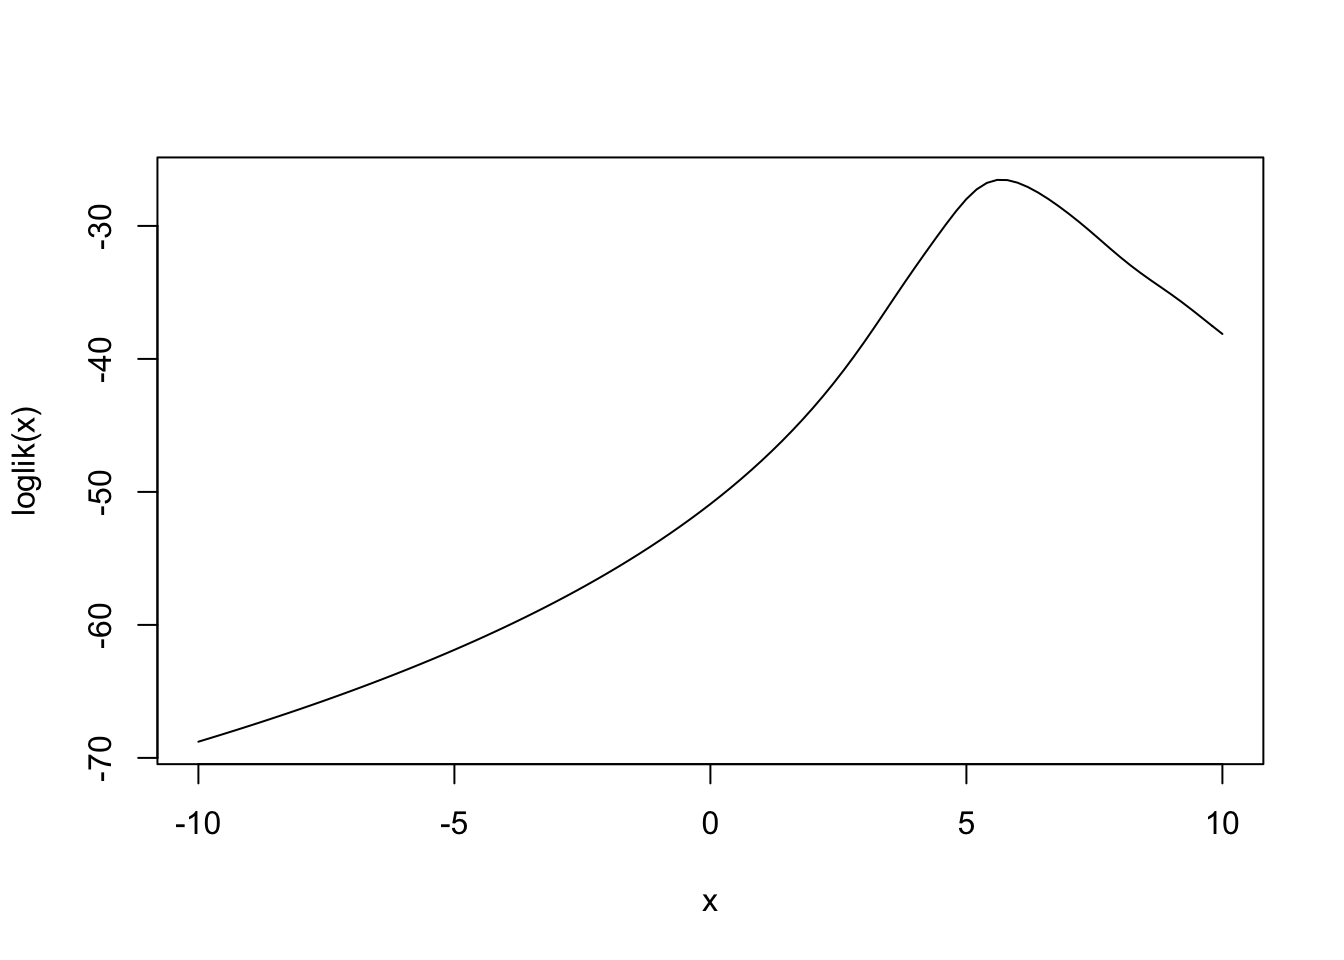
\includegraphics{Statistical-Computing-Solution_files/figure-latex/HW3_3-1.pdf}

\section{Newton-Raphson method}\label{newton-raphson-method}

\begin{Shaded}
\begin{Highlighting}[]
\KeywordTok{library}\NormalTok{(pracma)}
\NormalTok{## define the derivitive function}
\NormalTok{dev.loglik <-}\StringTok{ }\ControlFlowTok{function}\NormalTok{(theta) \{}
\NormalTok{  dev.l <-}\StringTok{ }\OperatorTok{-}\DecValTok{2} \OperatorTok{*}\StringTok{ }\KeywordTok{sum}\NormalTok{((theta}\OperatorTok{-}\NormalTok{X)}\OperatorTok{/}\NormalTok{(}\DecValTok{1}\OperatorTok{+}\NormalTok{(theta}\OperatorTok{-}\NormalTok{X)}\OperatorTok{^}\DecValTok{2}\NormalTok{))}
\NormalTok{  dev.l}
\NormalTok{\}}
\NormalTok{## define the hessian function}
\NormalTok{hessian.loglik <-}\StringTok{ }\ControlFlowTok{function}\NormalTok{(theta) \{}
\NormalTok{  h <-}\StringTok{ }\OperatorTok{-}\DecValTok{2} \OperatorTok{*}\StringTok{ }\KeywordTok{sum}\NormalTok{((}\DecValTok{1}\OperatorTok{-}\NormalTok{(theta}\OperatorTok{-}\NormalTok{X)}\OperatorTok{^}\DecValTok{2}\NormalTok{) }\OperatorTok{*}\StringTok{ }\NormalTok{(}\DecValTok{1}\OperatorTok{+}\NormalTok{(theta}\OperatorTok{-}\NormalTok{X)}\OperatorTok{^}\DecValTok{2}\NormalTok{)}\OperatorTok{^}\NormalTok{(}\OperatorTok{-}\DecValTok{2}\NormalTok{))}
\NormalTok{  h}
\NormalTok{\}}
\NormalTok{x0 <-}\StringTok{ }\KeywordTok{seq}\NormalTok{(}\OperatorTok{-}\DecValTok{10}\NormalTok{, }\DecValTok{20}\NormalTok{, }\DataTypeTok{by =} \FloatTok{0.5}\NormalTok{)}
\NormalTok{root.newton <-}\StringTok{ }\KeywordTok{rep}\NormalTok{(}\DecValTok{0}\NormalTok{, }\KeywordTok{length}\NormalTok{(x0))}
\ControlFlowTok{for}\NormalTok{ (i }\ControlFlowTok{in} \DecValTok{1}\OperatorTok{:}\KeywordTok{length}\NormalTok{(x0)) \{}
\NormalTok{  root.newton[i] <-}\StringTok{ }\KeywordTok{newtonRaphson}\NormalTok{(dev.loglik, }\DataTypeTok{x0 =}\NormalTok{ x0[i], }\DataTypeTok{dfun =}\NormalTok{ hessian.loglik)}\OperatorTok{$}\NormalTok{root}
\NormalTok{\}}
\KeywordTok{plot}\NormalTok{(x0, root.newton)}
\KeywordTok{abline}\NormalTok{(}\DataTypeTok{h =} \FloatTok{5.442}\NormalTok{)}
\end{Highlighting}
\end{Shaded}

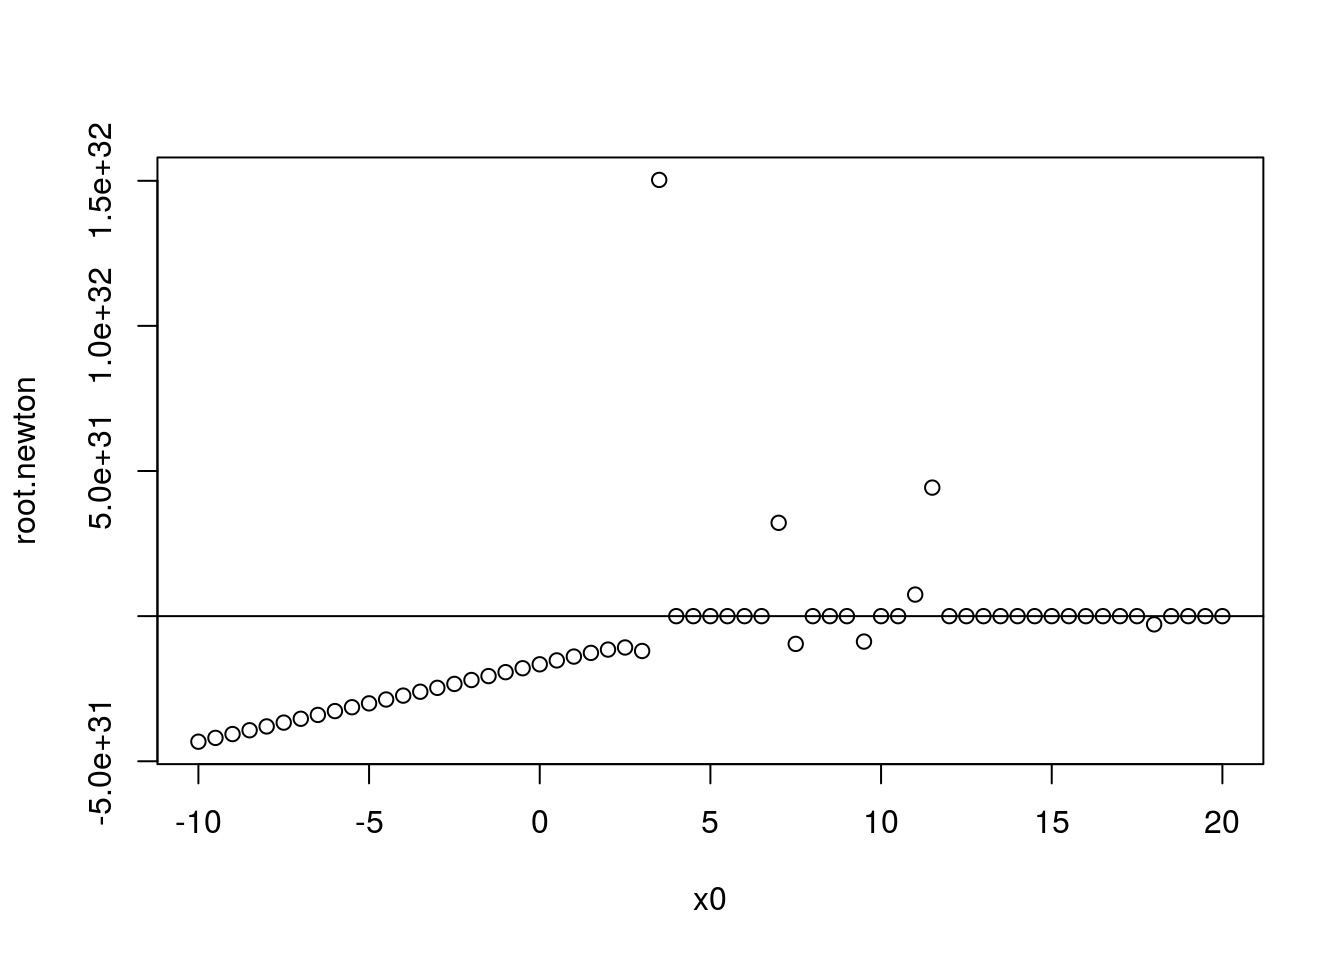
\includegraphics{Statistical-Computing-Solution_files/figure-latex/HW3_4-1.pdf}

\begin{Shaded}
\begin{Highlighting}[]
\NormalTok{root.newton}
\end{Highlighting}
\end{Shaded}

\begin{verbatim}
##  [1] -4.324741e+31 -4.193577e+31 -4.062249e+31 -3.930748e+31 -3.799064e+31
##  [6] -3.667185e+31 -3.535100e+31 -3.402796e+31 -3.270261e+31 -3.137479e+31
## [11] -3.004436e+31 -2.871118e+31 -2.737510e+31 -2.603599e+31 -2.469374e+31
## [16] -2.334832e+31 -2.199981e+31 -2.064850e+31 -1.929508e+31 -1.794100e+31
## [21] -1.658922e+31 -1.524582e+31 -1.392396e+31 -1.265439e+31 -1.151924e+31
## [26] -1.079358e+31 -1.199750e+31  1.502957e+32  2.056366e+01  2.108229e+01
## [31]  5.685422e+00  5.685422e+00  5.685422e+00  5.685422e+00  3.215974e+31
## [36] -9.558888e+30  1.937744e+01  2.108229e+01  5.685422e+00 -8.759488e+30
## [41]  2.108229e+01  5.685422e+00  7.439560e+30  4.429077e+31  2.056366e+01
## [46]  2.056366e+01  2.056366e+01  2.108229e+01  2.108229e+01  2.108230e+01
## [51]  1.937743e+01  2.056366e+01  2.056366e+01  1.937744e+01  1.937743e+01
## [56]  1.937744e+01 -2.825479e+30  2.056366e+01  2.056366e+01  2.056366e+01
## [61]  2.056366e+01
\end{verbatim}

We can see that Newton method doesn't converge when initial value is not
close to the real root.

\section{Fixed point method}\label{fixed-point-method}

\begin{Shaded}
\begin{Highlighting}[]
\NormalTok{## self-defined fixed point methods to find mle}
\NormalTok{## input gradiant of loglikelihood function, x0 is initial value}
\NormalTok{FixPoint.mle <-}\StringTok{ }\ControlFlowTok{function}\NormalTok{(dev.loglik, alpha, x0, }\DataTypeTok{maxiter =} \DecValTok{100}\NormalTok{, }
                     \DataTypeTok{tol =}\NormalTok{ .Machine}\OperatorTok{$}\NormalTok{double.eps}\OperatorTok{^}\FloatTok{0.5}\NormalTok{)\{}
\NormalTok{  x <-}\StringTok{ }\NormalTok{x0}
  \ControlFlowTok{for}\NormalTok{ (i }\ControlFlowTok{in} \DecValTok{1}\OperatorTok{:}\NormalTok{maxiter) \{}
\NormalTok{   x.new <-}\StringTok{ }\NormalTok{alpha }\OperatorTok{*}\StringTok{ }\KeywordTok{dev.loglik}\NormalTok{(x) }\OperatorTok{+}\StringTok{ }\NormalTok{x}
   \ControlFlowTok{if}\NormalTok{ (}\KeywordTok{abs}\NormalTok{(x.new }\OperatorTok{-}\StringTok{ }\NormalTok{x) }\OperatorTok{<}\StringTok{ }\NormalTok{tol) }\ControlFlowTok{break}
\NormalTok{   x <-}\StringTok{ }\NormalTok{x.new}
\NormalTok{  \}}
  \ControlFlowTok{if}\NormalTok{ (i }\OperatorTok{==}\StringTok{ }\NormalTok{maxiter) }\KeywordTok{warning}\NormalTok{(}\StringTok{"maximum iteration has reached"}\NormalTok{)}
  \KeywordTok{return}\NormalTok{(}\KeywordTok{list}\NormalTok{(}\DataTypeTok{root =}\NormalTok{ x, }\DataTypeTok{niter =}\NormalTok{ i))}
\NormalTok{\}}
\NormalTok{alpha <-}\StringTok{ }\KeywordTok{c}\NormalTok{(}\DecValTok{1}\NormalTok{, }\FloatTok{0.64}\NormalTok{, }\FloatTok{0.25}\NormalTok{)}
\NormalTok{root.fixpoint <-}\StringTok{ }\KeywordTok{matrix}\NormalTok{(}\DecValTok{0}\NormalTok{, }\DataTypeTok{ncol =} \KeywordTok{length}\NormalTok{(alpha), }\DataTypeTok{nrow =} \KeywordTok{length}\NormalTok{(x0))}
\ControlFlowTok{for}\NormalTok{ (i }\ControlFlowTok{in} \DecValTok{1}\OperatorTok{:}\KeywordTok{length}\NormalTok{(alpha)) \{}
  \ControlFlowTok{for}\NormalTok{ (j }\ControlFlowTok{in} \DecValTok{1}\OperatorTok{:}\KeywordTok{length}\NormalTok{(x0)) \{}
\NormalTok{    root.fixpoint[j, i] <-}\StringTok{ }\KeywordTok{FixPoint.mle}\NormalTok{(}\DataTypeTok{dev.loglik =}\NormalTok{ dev.loglik, }\DataTypeTok{alpha =}\NormalTok{ alpha[i], }
                                        \DataTypeTok{x0 =}\NormalTok{ x0[j])}\OperatorTok{$}\NormalTok{root}
\NormalTok{  \}}
\NormalTok{\}}
\KeywordTok{plot}\NormalTok{(x0, root.fixpoint[, }\DecValTok{1}\NormalTok{], }\DataTypeTok{ylim =} \KeywordTok{c}\NormalTok{(}\KeywordTok{min}\NormalTok{(root.fixpoint), }\KeywordTok{max}\NormalTok{(root.fixpoint)), }
     \DataTypeTok{ylab =} \StringTok{"root"}\NormalTok{, }\DataTypeTok{xlab =} \StringTok{"initial value"}\NormalTok{, }
     \DataTypeTok{main =} \KeywordTok{paste0}\NormalTok{(}\StringTok{"black: "}\NormalTok{, }\KeywordTok{expression}\NormalTok{(alpha), }\StringTok{"= 1; red: "}\NormalTok{, }\KeywordTok{expression}\NormalTok{(alpha), }
     \StringTok{"= 0.64; green: "}\NormalTok{, }\KeywordTok{expression}\NormalTok{(alpha), }\StringTok{"= 0.25"}\NormalTok{))}
\KeywordTok{points}\NormalTok{(x0, root.fixpoint[, }\DecValTok{2}\NormalTok{], }\DataTypeTok{col =} \StringTok{"red"}\NormalTok{)}
\KeywordTok{points}\NormalTok{(x0, root.fixpoint[, }\DecValTok{3}\NormalTok{], }\DataTypeTok{col =} \StringTok{"green"}\NormalTok{)}
\end{Highlighting}
\end{Shaded}

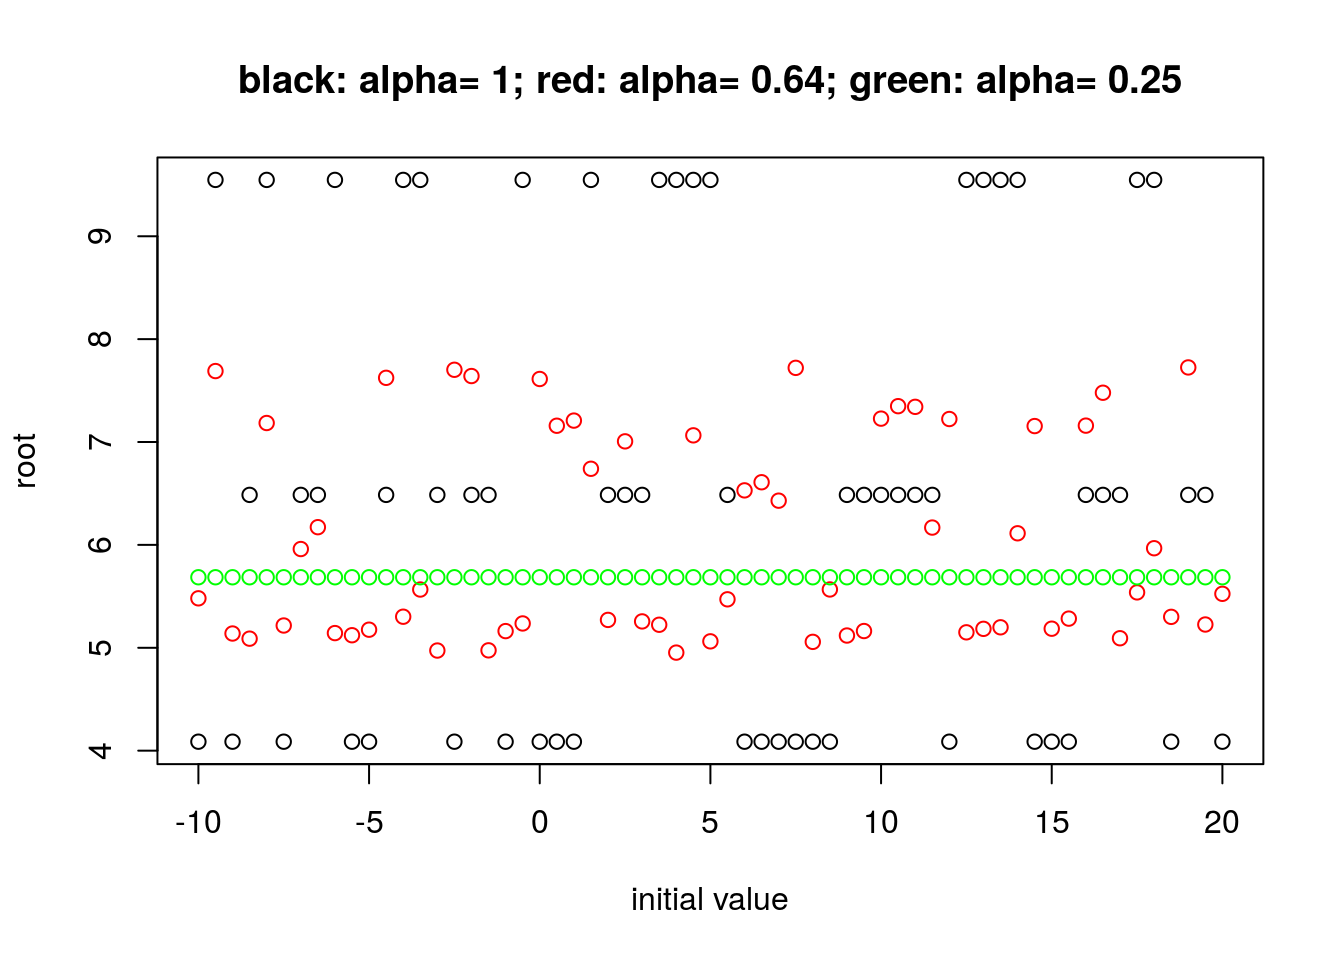
\includegraphics{Statistical-Computing-Solution_files/figure-latex/HW3_5-1.pdf}

\section{Fisher scoring and
Newton-Raphson}\label{fisher-scoring-and-newton-raphson}

\begin{Shaded}
\begin{Highlighting}[]
\NormalTok{## Self-defined fisher scoring method to find mle.}
\NormalTok{## input gradiant of loglikelihood and sample fisher information.}
\NormalTok{FisherScore.mle <-}\StringTok{ }\ControlFlowTok{function}\NormalTok{(dev.loglik, information, x0, }\DataTypeTok{maxiter =} \DecValTok{100}\NormalTok{,}
                            \DataTypeTok{tol =}\NormalTok{ .Machine}\OperatorTok{$}\NormalTok{double.eps}\OperatorTok{^}\FloatTok{0.5}\NormalTok{) \{}
\NormalTok{  x <-}\StringTok{ }\NormalTok{x0}
  \ControlFlowTok{for}\NormalTok{ (i }\ControlFlowTok{in} \DecValTok{1}\OperatorTok{:}\NormalTok{maxiter) \{}
\NormalTok{    x.new <-}\StringTok{ }\NormalTok{x }\OperatorTok{+}\StringTok{ }\KeywordTok{dev.loglik}\NormalTok{(x) }\OperatorTok{/}\StringTok{ }\KeywordTok{information}\NormalTok{(x)}
    \ControlFlowTok{if}\NormalTok{ (}\KeywordTok{abs}\NormalTok{(x.new }\OperatorTok{-}\StringTok{ }\NormalTok{x) }\OperatorTok{<}\StringTok{ }\NormalTok{tol) }\ControlFlowTok{break}
\NormalTok{    x <-}\StringTok{ }\NormalTok{x.new}
\NormalTok{   \}}
   \ControlFlowTok{if}\NormalTok{ (i }\OperatorTok{==}\StringTok{ }\NormalTok{maxiter) }\KeywordTok{warning}\NormalTok{(}\StringTok{"maximum iteration has reached"}\NormalTok{)}
   \KeywordTok{return}\NormalTok{(}\KeywordTok{list}\NormalTok{(}\DataTypeTok{root =}\NormalTok{ x, }\DataTypeTok{niter =}\NormalTok{ i))}
\NormalTok{\}}
\NormalTok{FisherNewton.mle <-}\StringTok{ }\ControlFlowTok{function}\NormalTok{(dev.loglik, information, dfun, x0, }\DataTypeTok{maxiter =} \DecValTok{100}\NormalTok{, }
                             \DataTypeTok{tol =}\NormalTok{ .Machine}\OperatorTok{$}\NormalTok{double.eps}\OperatorTok{^}\FloatTok{0.5}\NormalTok{) \{}
\NormalTok{  method.fisher <-}\StringTok{ }\KeywordTok{FisherScore.mle}\NormalTok{(}\DataTypeTok{dev.loglik =}\NormalTok{ dev.loglik, }\DataTypeTok{information =}\NormalTok{ information, }
                              \DataTypeTok{x0 =}\NormalTok{ x0, }\DataTypeTok{maxiter =}\NormalTok{ maxiter, }\DataTypeTok{tol =}\NormalTok{ tol)}
\NormalTok{  x.fisher <-}\StringTok{ }\NormalTok{method.fisher}\OperatorTok{$}\NormalTok{root}
\NormalTok{  niter.fisher <-}\StringTok{ }\NormalTok{method.fisher}\OperatorTok{$}\NormalTok{niter}
\NormalTok{  method.newton <-}\StringTok{ }\KeywordTok{newtonRaphson}\NormalTok{(}\DataTypeTok{fun =}\NormalTok{ dev.loglik, }\DataTypeTok{x0 =}\NormalTok{ x.fisher, }\DataTypeTok{dfun =}\NormalTok{ dfun, }\DataTypeTok{maxiter =}\NormalTok{ maxiter, }
                        \DataTypeTok{tol =}\NormalTok{ tol)}
  \KeywordTok{return}\NormalTok{(}\KeywordTok{list}\NormalTok{(}\DataTypeTok{root =}\NormalTok{ method.newton}\OperatorTok{$}\NormalTok{root, }\DataTypeTok{niter.fisher =}\NormalTok{ niter.fisher, }
              \DataTypeTok{niter.newton =}\NormalTok{ method.newton}\OperatorTok{$}\NormalTok{niter))}
\NormalTok{\}}
\NormalTok{inf.cauchy <-}\StringTok{ }\ControlFlowTok{function}\NormalTok{(x) n}\OperatorTok{/}\DecValTok{2}

\NormalTok{root.mix <-}\StringTok{ }\KeywordTok{rep}\NormalTok{(}\DecValTok{0}\NormalTok{, }\KeywordTok{length}\NormalTok{(x0))}
\ControlFlowTok{for}\NormalTok{ (i }\ControlFlowTok{in} \DecValTok{1}\OperatorTok{:}\KeywordTok{length}\NormalTok{(x0)) \{}
\NormalTok{  root.mix[i] <-}\StringTok{ }\KeywordTok{FisherNewton.mle}\NormalTok{(dev.loglik, inf.cauchy, }\DataTypeTok{dfun =}\NormalTok{ hessian.loglik, }
                                  \DataTypeTok{x0 =}\NormalTok{ x0[i])}\OperatorTok{$}\NormalTok{root}
\NormalTok{\}}
\KeywordTok{plot}\NormalTok{(x0, root.mix)}
\end{Highlighting}
\end{Shaded}

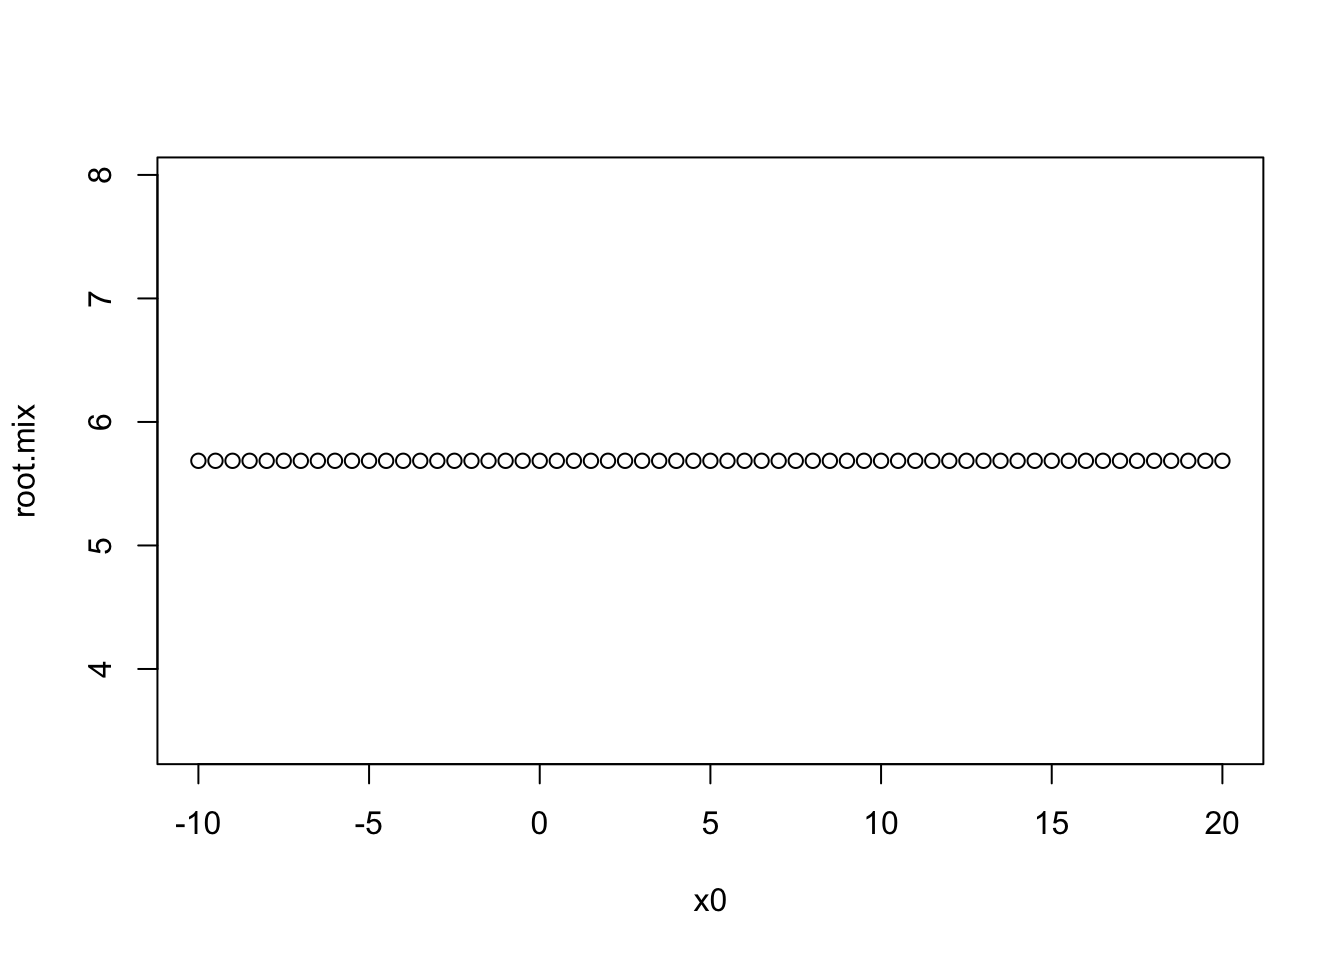
\includegraphics{Statistical-Computing-Solution_files/figure-latex/HW3_6-1.pdf}

\section{comparing the different
methods}\label{comparing-the-different-methods}

\begin{Shaded}
\begin{Highlighting}[]
\KeywordTok{library}\NormalTok{(microbenchmark)}
\NormalTok{## comparing the speed of different methods}
\NormalTok{## use starting point 5, alpha = 0.25 for fixed point method}
\NormalTok{newton.method <-}\StringTok{ }\KeywordTok{newtonRaphson}\NormalTok{(}\DataTypeTok{fun =}\NormalTok{ dev.loglik, }\DataTypeTok{x0 =} \DecValTok{5}\NormalTok{, }\DataTypeTok{dfun =}\NormalTok{ hessian.loglik)}
\NormalTok{fixpoint.method <-}\StringTok{ }\KeywordTok{FixPoint.mle}\NormalTok{(}\DataTypeTok{dev.loglik =}\NormalTok{ dev.loglik, }\DataTypeTok{alpha =} \FloatTok{0.25}\NormalTok{, }\DataTypeTok{x0 =} \DecValTok{5}\NormalTok{)}
\NormalTok{fishernewton.method <-}\StringTok{ }\KeywordTok{FisherNewton.mle}\NormalTok{(}\DataTypeTok{dev.loglik =}\NormalTok{ dev.loglik, }\DataTypeTok{information =}\NormalTok{ inf.cauchy, }
                                \DataTypeTok{dfun =}\NormalTok{ hessian.loglik, }\DataTypeTok{x0 =} \DecValTok{5}\NormalTok{)}
\KeywordTok{list}\NormalTok{(}\DataTypeTok{newton.niter =}\NormalTok{ newton.method}\OperatorTok{$}\NormalTok{niter, }\DataTypeTok{fixpoint.niter =}\NormalTok{ fixpoint.method}\OperatorTok{$}\NormalTok{niter, }
     \DataTypeTok{fishernewton.niter =} \KeywordTok{c}\NormalTok{(fishernewton.method}\OperatorTok{$}\NormalTok{niter.fisher, }
\NormalTok{                            fishernewton.method}\OperatorTok{$}\NormalTok{niter.newton))}
\end{Highlighting}
\end{Shaded}

\begin{verbatim}
## $newton.niter
## [1] 6
## 
## $fixpoint.niter
## [1] 17
## 
## $fishernewton.niter
## [1] 8 1
\end{verbatim}

Fixed point method is most stable but converges slowly compare to the
other two methods. Newton-Raphson methods converges fastest but is the
most unstably one. Fisher-Scoring converges slower than Newton, but is
very stable and accuracy, after refining with Newton-Raphson methods.
Also we can see that if we use fisher scoring root to be the initial
value of Newton-Raphson method, it will converge very fast.

\chapter{Exercise 3.2}\label{exercise-3.2}

\section{Find the the log-likelihood
function}\label{find-the-the-log-likelihood-function}

The log-likelihood function of this distribution is

\[ \ell(\mathbf{x}, \theta) = \sum_{i=1}^n \log\{1-\cos(x_i-\theta)\} - n\log2\pi\]

\begin{Shaded}
\begin{Highlighting}[]
\NormalTok{x <-}\StringTok{ }\KeywordTok{c}\NormalTok{(}\FloatTok{3.91}\NormalTok{, }\FloatTok{4.85}\NormalTok{, }\FloatTok{2.28}\NormalTok{, }\FloatTok{4.06}\NormalTok{, }\FloatTok{3.70}\NormalTok{, }\FloatTok{4.04}\NormalTok{, }\FloatTok{5.46}\NormalTok{, }\FloatTok{3.53}\NormalTok{, }\FloatTok{2.28}\NormalTok{, }\FloatTok{1.96}\NormalTok{,}
       \FloatTok{2.53}\NormalTok{, }\FloatTok{3.88}\NormalTok{, }\FloatTok{2.22}\NormalTok{, }\FloatTok{3.47}\NormalTok{, }\FloatTok{4.82}\NormalTok{, }\FloatTok{2.46}\NormalTok{, }\FloatTok{2.99}\NormalTok{, }\FloatTok{2.54}\NormalTok{, }\FloatTok{0.52}\NormalTok{)}

\NormalTok{loglikelihood <-}\StringTok{ }\ControlFlowTok{function}\NormalTok{(theta)\{}
\NormalTok{  n <-}\StringTok{ }\KeywordTok{length}\NormalTok{(x)}
\NormalTok{  s <-}\StringTok{ }\KeywordTok{sum}\NormalTok{(}\KeywordTok{log}\NormalTok{(}\DecValTok{1} \OperatorTok{-}\StringTok{ }\KeywordTok{cos}\NormalTok{(x }\OperatorTok{-}\StringTok{ }\NormalTok{theta))) }\OperatorTok{+}\StringTok{ }\NormalTok{n }\OperatorTok{*}\StringTok{ }\KeywordTok{log}\NormalTok{(}\DecValTok{2} \OperatorTok{*}\StringTok{ }\NormalTok{pi)}
  \KeywordTok{return}\NormalTok{(s)}
\NormalTok{\}}
\NormalTok{loglikelihood <-}\StringTok{ }\KeywordTok{Vectorize}\NormalTok{(loglikelihood)}
\KeywordTok{curve}\NormalTok{(loglikelihood, }\OperatorTok{-}\NormalTok{pi, pi, }\DataTypeTok{xlab =} \KeywordTok{expression}\NormalTok{(theta), }\DataTypeTok{ylab =} \StringTok{"log-likelihood"}\NormalTok{)}
\end{Highlighting}
\end{Shaded}

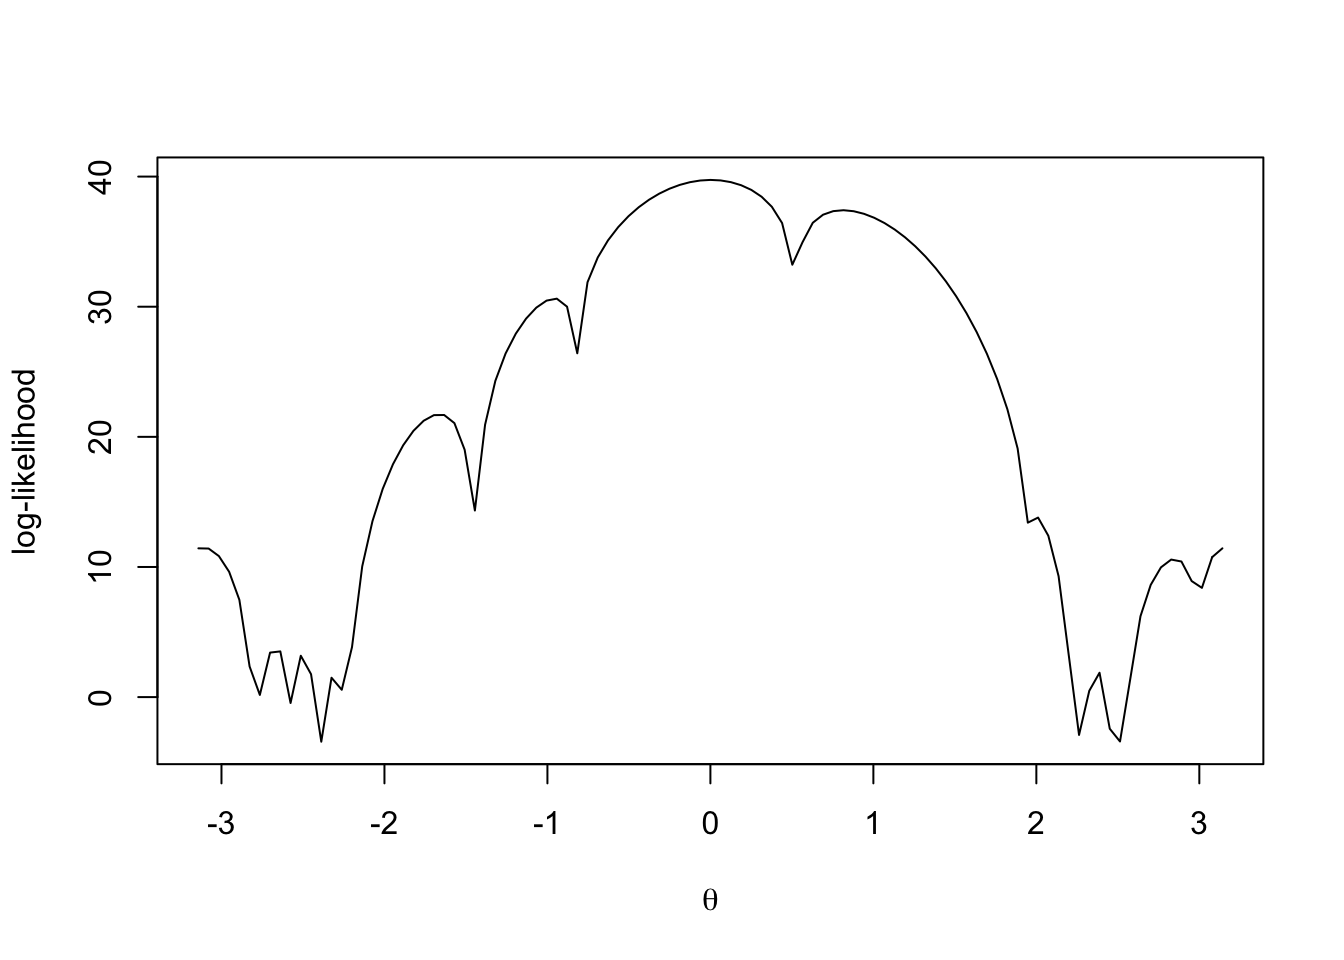
\includegraphics{Statistical-Computing-Solution_files/figure-latex/unnamed-chunk-2-1.pdf}

\section{Find the method-of-moments
estimator}\label{find-the-method-of-moments-estimator}

The expectation of \(\mathbf{x}|\theta\) is

\begin{align*}
\mathbb E (x | \theta) &= \int_{0}^{2\pi} x \frac{1-\cos(x-\theta)}{2\pi} dx \\
&= \frac{1}{2\pi} \int_{0}^{2\pi} x - x\cos(x-\theta) dx \\
&= \pi + \sin(\theta) \\
&= \bar{X_n}
\end{align*}

Thus,

\begin{Shaded}
\begin{Highlighting}[]
\NormalTok{theta_tilde <-}\StringTok{ }\KeywordTok{asin}\NormalTok{(}\KeywordTok{mean}\NormalTok{(x) }\OperatorTok{-}\StringTok{ }\NormalTok{pi)}
\NormalTok{theta_tilde}
\end{Highlighting}
\end{Shaded}

\begin{verbatim}
## [1] 0.09539407
\end{verbatim}

\section{Find the MLE}\label{find-the-mle}

Since

\[\frac{\partial\ell(\mathbf{x}; \theta)}{\partial\theta} = \sum_{i=1}^n \frac{-\sin(x_i - \theta)}{1-\cos(x_i-\theta)}\]

\[\frac{\partial^2\ell(\mathbf{x}; \theta)}{\partial \theta^2} = \sum_{i=1}^n \frac{\cos(x_i-\theta) - \cos^2(x_i-\theta)-\sin^2(x_i-\theta)}{(1-\cos(x_i-\theta))^2}\]

The Newton-Raphson method is

\[\hat\theta^{(t+1)} = \hat\theta^{(t)} - \left\{\frac{\partial^2\ell(\mathbf{x}; \hat\theta^{(t)})}{\partial \theta^2}\right\}^{-1}\frac{\partial\ell(\mathbf{x}; \hat\theta^{(t)})}{\partial\theta}\]

\begin{Shaded}
\begin{Highlighting}[]
\NormalTok{lfd <-}\StringTok{ }\ControlFlowTok{function}\NormalTok{(theta)\{}
  \KeywordTok{sum}\NormalTok{(}\OperatorTok{-}\KeywordTok{sin}\NormalTok{(x}\OperatorTok{-}\NormalTok{theta)}\OperatorTok{/}\NormalTok{(}\DecValTok{1}\OperatorTok{-}\KeywordTok{cos}\NormalTok{(x}\OperatorTok{-}\NormalTok{theta)))}
\NormalTok{\}}

\NormalTok{lsd <-}\StringTok{ }\ControlFlowTok{function}\NormalTok{(theta)\{}
  \KeywordTok{sum}\NormalTok{((}\KeywordTok{cos}\NormalTok{(x}\OperatorTok{-}\NormalTok{theta) }\OperatorTok{-}\StringTok{ }\NormalTok{(}\KeywordTok{cos}\NormalTok{(x}\OperatorTok{-}\NormalTok{theta))}\OperatorTok{^}\DecValTok{2} \OperatorTok{-}\StringTok{ }\NormalTok{(}\KeywordTok{sin}\NormalTok{(x}\OperatorTok{-}\NormalTok{theta))}\OperatorTok{^}\DecValTok{2}\NormalTok{)}\OperatorTok{/}\NormalTok{(}\DecValTok{1}\OperatorTok{-}\KeywordTok{cos}\NormalTok{(x}\OperatorTok{-}\NormalTok{theta))}\OperatorTok{^}\DecValTok{2}\NormalTok{)}
\NormalTok{\}}

\NormalTok{Newton <-}\StringTok{ }\ControlFlowTok{function}\NormalTok{(init)\{}
\NormalTok{  theta0 <-}\StringTok{ }\NormalTok{init}
\NormalTok{  i <-}\StringTok{ }\DecValTok{0}
\NormalTok{  diff <-}\StringTok{ }\DecValTok{1}
\NormalTok{  msg <-}\StringTok{ "converge"}
  \ControlFlowTok{while}\NormalTok{(}\KeywordTok{abs}\NormalTok{(diff) }\OperatorTok{>}\StringTok{ }\FloatTok{0.0000001}\NormalTok{)\{}
\NormalTok{    lfd <-}\StringTok{ }\KeywordTok{lfd}\NormalTok{(theta0)}
\NormalTok{    lsd <-}\StringTok{ }\KeywordTok{lsd}\NormalTok{(theta0)}
\NormalTok{    diff <-}\StringTok{ }\NormalTok{(lfd}\OperatorTok{/}\NormalTok{lsd)}
\NormalTok{    theta1 <-}\StringTok{ }\NormalTok{theta0 }\OperatorTok{-}\StringTok{ }\NormalTok{diff}
\NormalTok{    theta0 <-}\StringTok{ }\NormalTok{theta1}
\NormalTok{    i <-}\StringTok{ }\NormalTok{i}\OperatorTok{+}\DecValTok{1}
    \CommentTok{#cat(i)}
    \ControlFlowTok{if}\NormalTok{(i }\OperatorTok{>=}\StringTok{ }\DecValTok{150}\NormalTok{)\{}
\NormalTok{      msg <-}\StringTok{ "Not converge"}
\NormalTok{      theta0 <-}\StringTok{ }\OtherTok{Inf}
      \ControlFlowTok{break}
\NormalTok{    \}}
\NormalTok{  \}}
  \KeywordTok{return}\NormalTok{(}\KeywordTok{list}\NormalTok{(}\DataTypeTok{theta =}\NormalTok{ theta0, }\DataTypeTok{itr =}\NormalTok{ i, }\DataTypeTok{msg =}\NormalTok{ msg))}
\NormalTok{\}}
\KeywordTok{Newton}\NormalTok{(theta_tilde)}
\end{Highlighting}
\end{Shaded}

\begin{verbatim}
## $theta
## [1] 0.003118157
## 
## $itr
## [1] 4
## 
## $msg
## [1] "converge"
\end{verbatim}

\section{\texorpdfstring{\(\theta_0 = 2.7\) or
\(\theta_0 = -2.7\)}{\textbackslash{}theta\_0 = 2.7 or \textbackslash{}theta\_0 = -2.7}}\label{theta_0-2.7-or-theta_0--2.7}

\begin{Shaded}
\begin{Highlighting}[]
\KeywordTok{Newton}\NormalTok{(}\OperatorTok{-}\FloatTok{2.7}\NormalTok{)}
\end{Highlighting}
\end{Shaded}

\begin{verbatim}
## $theta
## [1] -2.668857
## 
## $itr
## [1] 4
## 
## $msg
## [1] "converge"
\end{verbatim}

\begin{Shaded}
\begin{Highlighting}[]
\KeywordTok{Newton}\NormalTok{(}\FloatTok{2.7}\NormalTok{)}
\end{Highlighting}
\end{Shaded}

\begin{verbatim}
## $theta
## [1] 2.848415
## 
## $itr
## [1] 5
## 
## $msg
## [1] "converge"
\end{verbatim}

The \(\hat\theta\) we got is different.

\section{Repeat the above using 200 equally spaced starting
values}\label{repeat-the-above-using-200-equally-spaced-starting-values}

\begin{Shaded}
\begin{Highlighting}[]
\NormalTok{init <-}\StringTok{ }\KeywordTok{seq}\NormalTok{(}\OperatorTok{-}\NormalTok{pi, pi, }\DataTypeTok{length.out=}\DecValTok{200}\NormalTok{)}
\NormalTok{result <-}\StringTok{ }\OtherTok{NULL}
\ControlFlowTok{for}\NormalTok{(initi }\ControlFlowTok{in}\NormalTok{ init)\{}
\NormalTok{  result <-}\StringTok{ }\KeywordTok{rbind}\NormalTok{(result, }\KeywordTok{c}\NormalTok{(initi, }\KeywordTok{Newton}\NormalTok{(initi)}\OperatorTok{$}\NormalTok{theta))}
\NormalTok{\}}
\KeywordTok{colnames}\NormalTok{(result) <-}\StringTok{ }\KeywordTok{c}\NormalTok{(}\StringTok{"Initial_value"}\NormalTok{, }\StringTok{"theta_hat"}\NormalTok{)}
\KeywordTok{split}\NormalTok{(result, result[,}\DecValTok{2}\NormalTok{])}
\end{Highlighting}
\end{Shaded}

\begin{verbatim}
## $`-3.11247050669846`
##  [1] -3.141593 -3.110019 -3.078445 -3.046871 -3.015297 -2.983724 -2.952150
##  [8] -2.920576 -2.889002 -2.857428 -2.825855 -3.112471 -3.112471 -3.112471
## [15] -3.112471 -3.112471 -3.112471 -3.112471 -3.112471 -3.112471 -3.112471
## [22] -3.112471
## 
## $`-2.78655685241805`
## [1] -2.794281 -2.786557
## 
## $`-2.78655685241804`
## [1] -2.762707 -2.786557
## 
## $`-2.66885745902142`
##  [1] -2.731133 -2.699560 -2.667986 -2.636412 -2.604838 -2.668857 -2.668857
##  [8] -2.668857 -2.668857 -2.668857
## 
## $`-2.50935603320277`
##  [1] -2.573264 -2.541691 -2.510117 -2.478543 -2.446969 -2.415395 -2.509356
##  [8] -2.509356 -2.509356 -2.509356 -2.509356 -2.509356
## 
## $`-2.38826662826452`
## [1] -2.383822 -2.388267
## 
## $`-2.29792596896698`
## [1] -2.352248 -2.297926
## 
## $`-2.29792596896697`
## [1] -2.320674 -2.289100 -2.257526 -2.297926 -2.297926 -2.297926
## 
## $`-2.23219189887219`
## [1] -2.225953 -2.232192
## 
## $`-1.66271239546243`
##  [1] -2.194379 -2.162805 -2.131231 -2.099657 -2.068084 -2.036510 -2.004936
##  [8] -1.973362 -1.941788 -1.910215 -1.878641 -1.847067 -1.815493 -1.783919
## [15] -1.752346 -1.720772 -1.689198 -1.594477 -1.531329 -1.499755 -1.468181
## [22] -1.662712 -1.662712 -1.662712 -1.662712 -1.662712 -1.662712 -1.662712
## [29] -1.662712 -1.662712 -1.662712 -1.662712 -1.662712 -1.662712 -1.662712
## [36] -1.662712 -1.662712 -1.662712 -1.662712 -1.662712 -1.662712 -1.662712
## 
## $`-1.66271239546242`
## [1] -1.657624 -1.626050 -1.562903 -1.662712 -1.662712 -1.662712
## 
## $`-1.44750255268373`
## [1] -1.436608 -1.447503
## 
## $`-0.95440583712848`
##  [1] -1.4050339 -1.3103125 -1.2787387 -1.2155911 -1.1208697 -1.0577221
##  [7] -1.0261484 -0.9945746 -0.9544058 -0.9544058 -0.9544058 -0.9544058
## [13] -0.9544058 -0.9544058 -0.9544058 -0.9544058
## 
## $`-0.954405837128479`
##  [1] -1.3734601 -1.3418863 -1.1524435 -1.0892959 -0.9630008 -0.8998532
##  [7] -0.8682794 -0.8367056 -0.9544058 -0.9544058 -0.9544058 -0.9544058
## [13] -0.9544058 -0.9544058 -0.9544058 -0.9544058
## 
## $`-0.954405837128476`
## [1] -0.9314270 -0.9544058
## 
## $`-0.95440583712847`
## [1] -1.2471649 -0.9544058
## 
## $`-0.954405837128466`
## [1] -1.1840173 -0.9544058
## 
## $`0.00311815708656577`
## [1] -0.489393830  0.003118157
## 
## $`0.0031181570865658`
## [1] -0.078934489  0.003118157
## 
## $`0.00311815708656581`
## [1] 0.110508284 0.003118157
## 
## $`0.00311815708656585`
## [1] -0.236803466  0.003118157
## 
## $`0.00311815708656587`
## [1] -0.142082080 -0.047360693  0.003118157  0.003118157
## 
## $`0.00311815708656589`
## [1] -0.678836604 -0.584115217  0.003118157  0.003118157
## 
## $`0.00311815708656591`
## [1] -0.110508284  0.015786898  0.003118157  0.003118157
## 
## $`0.00311815708656593`
## [1] -0.710410399  0.142082080  0.299951057  0.003118157  0.003118157
## [6]  0.003118157
## 
## $`0.00311815708656597`
## [1] -0.457820035  0.003118157
## 
## $`0.00311815708656598`
## [1] -0.015786898  0.236803466  0.268377262  0.003118157  0.003118157
## [6]  0.003118157
## 
## $`0.00311815708656599`
## [1] -0.805131786  0.003118157
## 
## $`0.003118157086566`
## [1] -0.741984195  0.003118157
## 
## $`0.00311815708656601`
## [1] -0.268377262  0.394672444  0.003118157  0.003118157
## 
## $`0.00311815708656602`
## [1] -0.647262808 -0.552541421  0.078934489  0.003118157  0.003118157
## [6]  0.003118157
## 
## $`0.00311815708656603`
## [1] -0.773557990 -0.615689013  0.047360693  0.489393830  0.003118157
## [6]  0.003118157  0.003118157  0.003118157
## 
## $`0.00311815708656604`
## [1] -0.363098648  0.003118157
## 
## $`0.00311815708656606`
## [1] 0.457820035 0.003118157
## 
## $`0.00311815708656607`
## [1] -0.426246239  0.003118157
## 
## $`0.00311815708656609`
## [1] -0.173655875  0.003118157
## 
## $`0.00311815708656611`
## [1] -0.205229671  0.003118157
## 
## $`0.00311815708656612`
## [1] -0.394672444  0.363098648  0.003118157  0.003118157
## 
## $`0.00311815708656613`
## [1] -0.299951057  0.003118157
## 
## $`0.00311815708656615`
## [1] 0.205229671 0.003118157
## 
## $`0.00311815708656793`
## [1] 0.426246239 0.003118157
## 
## $`0.00311815708656861`
## [1] -0.520967626  0.003118157
## 
## $`0.00311815708656864`
## [1] 0.331524853 0.003118157
## 
## $`0.00311815708656926`
## [1] -0.331524853  0.003118157
## 
## $`0.00311815708656987`
## [1] 0.173655875 0.003118157
## 
## $`0.812637416717926`
## [1] 1.2787387 0.8126374
## 
## $`0.812637416717938`
## [1] 0.8051318 1.4050339 0.8126374 0.8126374
## 
## $`0.812637416717939`
## [1] 0.6788366 0.8126374
## 
## $`0.81263741671794`
##  [1] 0.5209676 0.5525414 0.5841152 0.6156890 0.6472628 0.7104104 0.7419842
##  [8] 0.7735580 0.8367056 0.8682794 0.8998532 0.9314270 0.9630008 0.9945746
## [15] 1.0261484 1.0577221 1.0892959 1.1208697 1.1524435 1.1840173 1.2155911
## [22] 1.2471649 1.3103125 1.3418863 1.3734601 1.4366077 1.4681815 1.4997553
## [29] 1.5313291 1.5629029 1.5944767 1.6260505 1.6576243 1.6891981 1.7207719
## [36] 1.7523457 1.7839194 1.8154932 1.8470670 1.8786408 1.9102146 1.9417884
## [43] 0.8126374 0.8126374 0.8126374 0.8126374 0.8126374 0.8126374 0.8126374
## [50] 0.8126374 0.8126374 0.8126374 0.8126374 0.8126374 0.8126374 0.8126374
## [57] 0.8126374 0.8126374 0.8126374 0.8126374 0.8126374 0.8126374 0.8126374
## [64] 0.8126374 0.8126374 0.8126374 0.8126374 0.8126374 0.8126374 0.8126374
## [71] 0.8126374 0.8126374 0.8126374 0.8126374 0.8126374 0.8126374 0.8126374
## [78] 0.8126374 0.8126374 0.8126374 0.8126374 0.8126374 0.8126374 0.8126374
## 
## $`2.00722323801594`
##  [1] 1.973362 2.004936 2.068084 2.099657 2.131231 2.162805 2.194379
##  [8] 2.007223 2.007223 2.007223 2.007223 2.007223 2.007223 2.007223
## 
## $`2.00722323801595`
## [1] 2.036510 2.007223
## 
## $`2.23701292270577`
## [1] 2.225953 2.257526 2.237013 2.237013
## 
## $`2.37471166606864`
##  [1] 2.289100 2.320674 2.352248 2.383822 2.415395 2.446969 2.374712
##  [8] 2.374712 2.374712 2.374712 2.374712 2.374712
## 
## $`2.48844965088485`
## [1] 2.478543 2.488450
## 
## $`2.48844965088489`
## [1] 2.510117 2.488450
## 
## $`2.84841532545741`
##  [1] 2.541691 2.573264 2.604838 2.636412 2.667986 2.699560 2.731133
##  [8] 2.762707 2.794281 2.825855 2.857428 2.920576 2.952150 2.983724
## [15] 2.848415 2.848415 2.848415 2.848415 2.848415 2.848415 2.848415
## [22] 2.848415 2.848415 2.848415 2.848415 2.848415 2.848415 2.848415
## 
## $`2.84841532545742`
## [1] 2.889002 2.848415
## 
## $`3.17071480048113`
##  [1] 3.015297 3.046871 3.078445 3.110019 3.141593 3.170715 3.170715
##  [8] 3.170715 3.170715 3.170715
\end{verbatim}

\chapter{Exercise 3.3}\label{exercise-3.3}

\section{Fit the population growth model to the beetles data using the
Gauss-Newton
approach}\label{fit-the-population-growth-model-to-the-beetles-data-using-the-gauss-newton-approach}

\begin{Shaded}
\begin{Highlighting}[]
\KeywordTok{library}\NormalTok{(graphics)}
\KeywordTok{library}\NormalTok{(Matrix)}
\NormalTok{beetles <-}\StringTok{ }\KeywordTok{data.frame}\NormalTok{(}
    \DataTypeTok{days    =} \KeywordTok{c}\NormalTok{(}\DecValTok{0}\NormalTok{,  }\DecValTok{8}\NormalTok{,  }\DecValTok{28}\NormalTok{,  }\DecValTok{41}\NormalTok{,  }\DecValTok{63}\NormalTok{,  }\DecValTok{69}\NormalTok{,   }\DecValTok{97}\NormalTok{, }\DecValTok{117}\NormalTok{,  }\DecValTok{135}\NormalTok{,  }\DecValTok{154}\NormalTok{),}
    \DataTypeTok{beetles =} \KeywordTok{c}\NormalTok{(}\DecValTok{2}\NormalTok{, }\DecValTok{47}\NormalTok{, }\DecValTok{192}\NormalTok{, }\DecValTok{256}\NormalTok{, }\DecValTok{768}\NormalTok{, }\DecValTok{896}\NormalTok{, }\DecValTok{1120}\NormalTok{, }\DecValTok{896}\NormalTok{, }\DecValTok{1184}\NormalTok{, }\DecValTok{1024}\NormalTok{))}

\NormalTok{##' define the sum of squared errors function}
\NormalTok{sqerr <-}\StringTok{ }\ControlFlowTok{function}\NormalTok{(k, r) \{}
\NormalTok{  s <-}\StringTok{ }\KeywordTok{matrix}\NormalTok{(}\DecValTok{0}\NormalTok{, }\DataTypeTok{nrow =} \KeywordTok{length}\NormalTok{(k), }\DataTypeTok{ncol =} \KeywordTok{length}\NormalTok{(r))}
  \ControlFlowTok{for}\NormalTok{ (i }\ControlFlowTok{in} \DecValTok{1}\OperatorTok{:}\KeywordTok{length}\NormalTok{(k)) \{}
    \ControlFlowTok{for}\NormalTok{ (j }\ControlFlowTok{in} \DecValTok{1}\OperatorTok{:}\KeywordTok{length}\NormalTok{(r)) \{}
\NormalTok{      s[i, j] <-}\StringTok{ }\KeywordTok{sum}\NormalTok{((beetles}\OperatorTok{$}\NormalTok{beetles }\OperatorTok{-}\StringTok{ }\NormalTok{k[i] }\OperatorTok{*}\StringTok{ }\NormalTok{beetles}\OperatorTok{$}\NormalTok{beetles[}\DecValTok{1}\NormalTok{] }\OperatorTok{/}\StringTok{ }
\StringTok{              }\NormalTok{(beetles}\OperatorTok{$}\NormalTok{beetles[}\DecValTok{1}\NormalTok{] }\OperatorTok{+}\StringTok{ }\NormalTok{(k[i] }\OperatorTok{-}\StringTok{ }\NormalTok{beetles}\OperatorTok{$}\NormalTok{beetles[}\DecValTok{1}\NormalTok{]) }\OperatorTok{*}\StringTok{ }
\StringTok{                 }\KeywordTok{exp}\NormalTok{(}\OperatorTok{-}\NormalTok{r[j]}\OperatorTok{*}\NormalTok{beetles}\OperatorTok{$}\NormalTok{days)))}\OperatorTok{^}\DecValTok{2}\NormalTok{)}
\NormalTok{    \}}
\NormalTok{  \}}
\NormalTok{  s}
\NormalTok{\}}

\NormalTok{##' define z function}
\NormalTok{z.vec <-}\StringTok{ }\ControlFlowTok{function}\NormalTok{(k, r) \{}
\NormalTok{  n <-}\StringTok{ }\KeywordTok{length}\NormalTok{(beetles}\OperatorTok{$}\NormalTok{days)}
\NormalTok{  z <-}\StringTok{ }\KeywordTok{rep}\NormalTok{(}\DecValTok{0}\NormalTok{, n)}
  \ControlFlowTok{for}\NormalTok{ (i }\ControlFlowTok{in} \DecValTok{1}\OperatorTok{:}\NormalTok{n) \{}
\NormalTok{   z[i] <-}\StringTok{ }\NormalTok{beetles}\OperatorTok{$}\NormalTok{beetles[i] }\OperatorTok{-}\StringTok{ }\NormalTok{k}\OperatorTok{*}\NormalTok{beetles}\OperatorTok{$}\NormalTok{beetles[}\DecValTok{1}\NormalTok{] }\OperatorTok{/}\StringTok{ }
\StringTok{     }\NormalTok{(beetles}\OperatorTok{$}\NormalTok{beetles[}\DecValTok{1}\NormalTok{] }\OperatorTok{+}\StringTok{ }\NormalTok{(k }\OperatorTok{-}\StringTok{ }\NormalTok{beetles}\OperatorTok{$}\NormalTok{beetles[}\DecValTok{1}\NormalTok{])}\OperatorTok{*}\KeywordTok{exp}\NormalTok{(}\OperatorTok{-}\NormalTok{r}\OperatorTok{*}\NormalTok{beetles}\OperatorTok{$}\NormalTok{days[i])) }
\NormalTok{  \}}
  \KeywordTok{return}\NormalTok{(z)}
\NormalTok{\}}

\NormalTok{##' define A matrix}
\NormalTok{A.mat <-}\StringTok{ }\ControlFlowTok{function}\NormalTok{(k, r) \{}
\NormalTok{  n <-}\StringTok{ }\KeywordTok{length}\NormalTok{(beetles}\OperatorTok{$}\NormalTok{days)}
\NormalTok{  A <-}\StringTok{ }\KeywordTok{matrix}\NormalTok{(}\DecValTok{0}\NormalTok{, }\DataTypeTok{nrow =}\NormalTok{ n, }\DataTypeTok{ncol =} \DecValTok{2}\NormalTok{)}
  \ControlFlowTok{for}\NormalTok{ (i }\ControlFlowTok{in} \DecValTok{1}\OperatorTok{:}\NormalTok{n) \{}
\NormalTok{    A[i, }\DecValTok{1}\NormalTok{] <-}\StringTok{ }\NormalTok{beetles}\OperatorTok{$}\NormalTok{beetles[}\DecValTok{1}\NormalTok{]}\OperatorTok{^}\DecValTok{2} \OperatorTok{*}\StringTok{ }\NormalTok{(}\DecValTok{1}\OperatorTok{-}\KeywordTok{exp}\NormalTok{(}\OperatorTok{-}\NormalTok{r}\OperatorTok{*}\NormalTok{beetles}\OperatorTok{$}\NormalTok{days[i])) }\OperatorTok{/}\StringTok{ }
\StringTok{      }\NormalTok{(beetles}\OperatorTok{$}\NormalTok{beetles[}\DecValTok{1}\NormalTok{] }\OperatorTok{+}\StringTok{ }\NormalTok{(k}\OperatorTok{-}\NormalTok{beetles}\OperatorTok{$}\NormalTok{beetles[}\DecValTok{1}\NormalTok{])}\OperatorTok{*}\KeywordTok{exp}\NormalTok{(}\OperatorTok{-}\NormalTok{r}\OperatorTok{*}\NormalTok{beetles}\OperatorTok{$}\NormalTok{days[i]))}\OperatorTok{^}\DecValTok{2}
    
\NormalTok{    A[i, }\DecValTok{2}\NormalTok{] <-}\StringTok{ }\NormalTok{beetles}\OperatorTok{$}\NormalTok{beetles[}\DecValTok{1}\NormalTok{]}\OperatorTok{*}\NormalTok{k}\OperatorTok{*}\NormalTok{beetles}\OperatorTok{$}\NormalTok{days[i]}\OperatorTok{*}\NormalTok{(k}\OperatorTok{-}\NormalTok{beetles}\OperatorTok{$}\NormalTok{beetles[}\DecValTok{1}\NormalTok{]) }\OperatorTok{*}\StringTok{ }
\StringTok{      }\KeywordTok{exp}\NormalTok{(}\OperatorTok{-}\NormalTok{r}\OperatorTok{*}\NormalTok{beetles}\OperatorTok{$}\NormalTok{days[i]) }\OperatorTok{/}\StringTok{ }\NormalTok{(beetles}\OperatorTok{$}\NormalTok{beetles[}\DecValTok{1}\NormalTok{]}\OperatorTok{+}\NormalTok{(k}\OperatorTok{-}\NormalTok{beetles}\OperatorTok{$}\NormalTok{beetles[}\DecValTok{1}\NormalTok{]) }\OperatorTok{*}\StringTok{ }
\StringTok{                                   }\KeywordTok{exp}\NormalTok{(}\OperatorTok{-}\NormalTok{r}\OperatorTok{*}\NormalTok{beetles}\OperatorTok{$}\NormalTok{days[i]))}\OperatorTok{^}\DecValTok{2}
\NormalTok{  \}}
  \KeywordTok{return}\NormalTok{(A)}
\NormalTok{\}}

\NormalTok{gaussNewton.beetles <-}\StringTok{ }\ControlFlowTok{function}\NormalTok{(para0, z.vec, A.mat, }\DataTypeTok{maxiter =} \DecValTok{100}\NormalTok{, }
                                \DataTypeTok{tol =}\NormalTok{ .Machine}\OperatorTok{$}\NormalTok{double.eps}\OperatorTok{^}\FloatTok{0.5}\NormalTok{) \{}
\NormalTok{  para <-}\StringTok{ }\NormalTok{para0}
  \ControlFlowTok{for}\NormalTok{ (i }\ControlFlowTok{in} \DecValTok{1}\OperatorTok{:}\NormalTok{maxiter) \{}
\NormalTok{    Amat <-}\StringTok{ }\KeywordTok{A.mat}\NormalTok{(para[}\DecValTok{1}\NormalTok{], para[}\DecValTok{2}\NormalTok{])}
\NormalTok{    zvec <-}\StringTok{ }\KeywordTok{z.vec}\NormalTok{(para[}\DecValTok{1}\NormalTok{], para[}\DecValTok{2}\NormalTok{])}
\NormalTok{    para.new <-}\StringTok{ }\NormalTok{para }\OperatorTok{+}\StringTok{ }\KeywordTok{solve}\NormalTok{(}\KeywordTok{t}\NormalTok{(Amat) }\OperatorTok\StringTok{ }\NormalTok{Amat }\OperatorTok{+}\StringTok{ }\FloatTok{0.0001}\OperatorTok{*}\KeywordTok{diag}\NormalTok{(}\DataTypeTok{nrow =} \DecValTok{2}\NormalTok{)) }\OperatorTok\StringTok{ }
\StringTok{      }\KeywordTok{t}\NormalTok{(Amat) }\OperatorTok\StringTok{ }\NormalTok{zvec}
    \ControlFlowTok{if}\NormalTok{ (}\KeywordTok{sum}\NormalTok{(}\KeywordTok{abs}\NormalTok{(para.new }\OperatorTok{-}\StringTok{ }\NormalTok{para)) }\OperatorTok{<}\StringTok{ }\NormalTok{tol) }\ControlFlowTok{break}
\NormalTok{    para <-}\StringTok{ }\NormalTok{para.new}
\NormalTok{  \}}
  \ControlFlowTok{if}\NormalTok{ (i }\OperatorTok{==}\StringTok{ }\NormalTok{maxiter) }\KeywordTok{warning}\NormalTok{(}\StringTok{"maximum iteration has reached"}\NormalTok{)}
  \KeywordTok{return}\NormalTok{(}\KeywordTok{list}\NormalTok{(}\DataTypeTok{root =}\NormalTok{ para, }\DataTypeTok{niter =}\NormalTok{ i))}
\NormalTok{\}}

\NormalTok{fit <-}\StringTok{ }\KeywordTok{gaussNewton.beetles}\NormalTok{(}\DataTypeTok{para0 =} \KeywordTok{c}\NormalTok{(}\DecValTok{1200}\NormalTok{, }\FloatTok{0.1}\NormalTok{), }\DataTypeTok{z.vec =}\NormalTok{ z.vec, }\DataTypeTok{A.mat =}\NormalTok{ A.mat)}
\NormalTok{fit}\OperatorTok{$}\NormalTok{root}
\end{Highlighting}
\end{Shaded}

\begin{verbatim}
##              [,1]
## [1,] 1049.4072443
## [2,]    0.1182684
\end{verbatim}

\begin{Shaded}
\begin{Highlighting}[]
\NormalTok{k <-}\StringTok{ }\KeywordTok{seq}\NormalTok{(}\DecValTok{100}\NormalTok{, }\DecValTok{1500}\NormalTok{, }\DataTypeTok{by =} \DecValTok{10}\NormalTok{)}
\NormalTok{r <-}\StringTok{ }\KeywordTok{seq}\NormalTok{(}\FloatTok{0.1}\NormalTok{, }\FloatTok{0.5}\NormalTok{, }\DataTypeTok{by =} \FloatTok{0.001}\NormalTok{)}
\NormalTok{z <-}\StringTok{ }\KeywordTok{sqerr}\NormalTok{(k, r)}
\KeywordTok{contour}\NormalTok{(k, r, z, }\DataTypeTok{xlab =} \StringTok{"k"}\NormalTok{, }\DataTypeTok{ylab =} \StringTok{"r"}\NormalTok{, }\DataTypeTok{main =} \StringTok{"contour plot for squared error"}\NormalTok{)}
\end{Highlighting}
\end{Shaded}

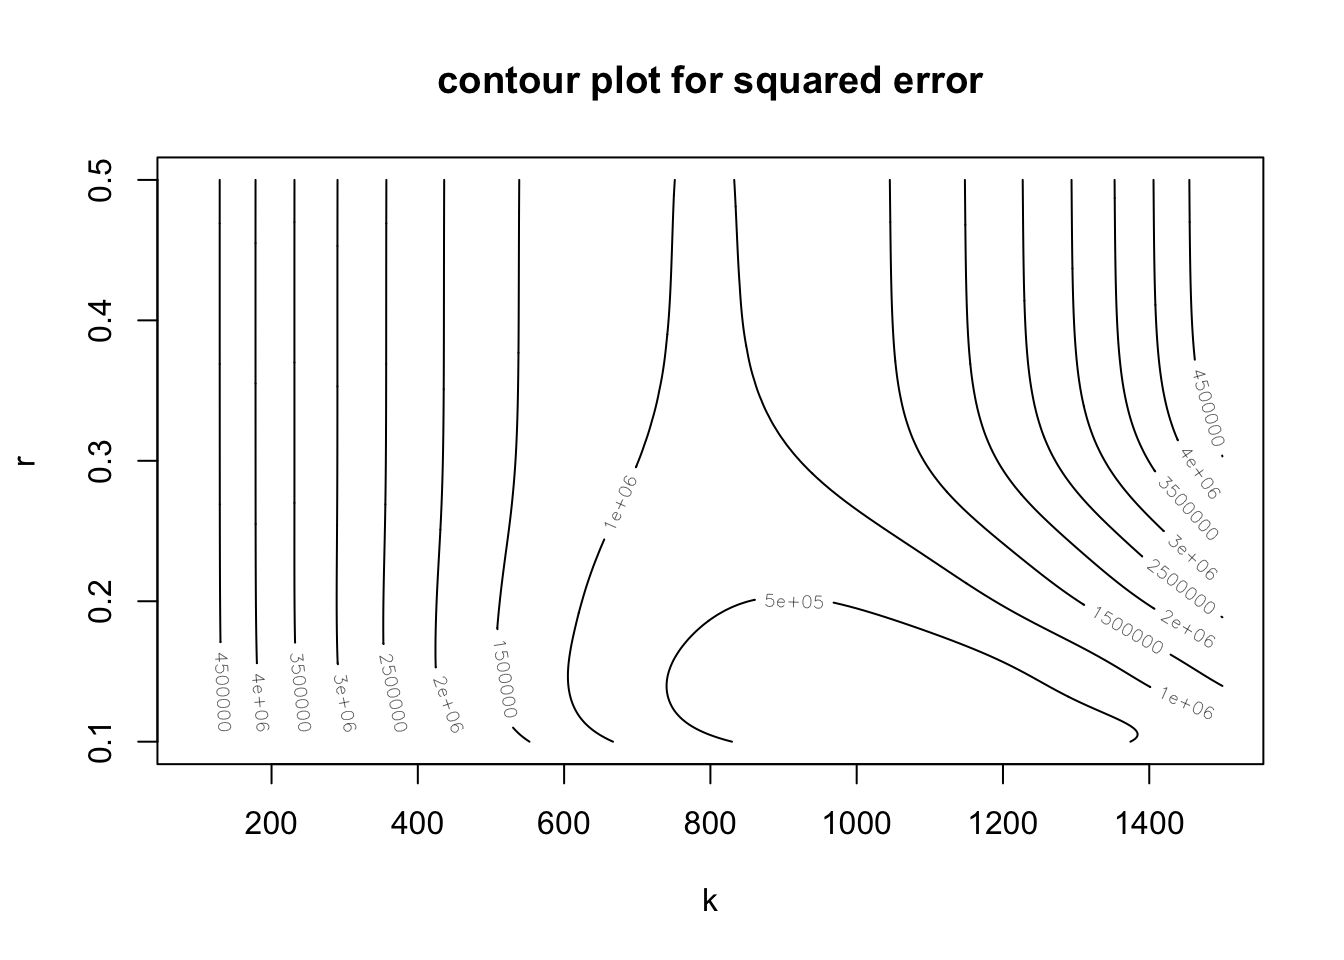
\includegraphics{Statistical-Computing-Solution_files/figure-latex/HW4_4-1.pdf}

Estimation using Gauss-Newton method is \(\hat{k} = 1049\),
\(\hat{r} = 0.12\).

\section{Log normal assumption}\label{log-normal-assumption}

\begin{Shaded}
\begin{Highlighting}[]
\NormalTok{##' define log-likelihood function}
\NormalTok{loglikeli <-}\StringTok{ }\ControlFlowTok{function}\NormalTok{(para) \{}
\NormalTok{  k <-}\StringTok{ }\NormalTok{para[}\DecValTok{1}\NormalTok{]}
\NormalTok{  r <-}\StringTok{ }\NormalTok{para[}\DecValTok{2}\NormalTok{]}
\NormalTok{  sigma2 <-}\StringTok{ }\NormalTok{para[}\DecValTok{3}\NormalTok{]}
\NormalTok{  l <-}\StringTok{ }\KeywordTok{sum}\NormalTok{(}\OperatorTok{-}\KeywordTok{log}\NormalTok{(}\DecValTok{2}\OperatorTok{*}\NormalTok{pi}\OperatorTok{*}\NormalTok{sigma2)}\OperatorTok{/}\DecValTok{2} \OperatorTok{-}\StringTok{ }\NormalTok{(}\KeywordTok{log}\NormalTok{(beetles}\OperatorTok{$}\NormalTok{beetles) }\OperatorTok{-}\StringTok{ }\KeywordTok{log}\NormalTok{(k) }\OperatorTok{-}\StringTok{ }
\StringTok{                                    }\KeywordTok{log}\NormalTok{(beetles}\OperatorTok{$}\NormalTok{beetles[}\DecValTok{1}\NormalTok{]) }\OperatorTok{+}\StringTok{ }
\StringTok{                                    }\KeywordTok{log}\NormalTok{(beetles}\OperatorTok{$}\NormalTok{beetles[}\DecValTok{1}\NormalTok{] }\OperatorTok{+}\StringTok{ }
\StringTok{                                          }\NormalTok{(k}\OperatorTok{-}\NormalTok{beetles}\OperatorTok{$}\NormalTok{beetles[}\DecValTok{1}\NormalTok{]) }\OperatorTok{*}\StringTok{ }
\StringTok{                                          }\KeywordTok{exp}\NormalTok{(}\OperatorTok{-}\NormalTok{r}\OperatorTok{*}\NormalTok{beetles}\OperatorTok{$}\NormalTok{days))}\OperatorTok{^}\DecValTok{2}\NormalTok{)}\OperatorTok{/}\DecValTok{2}\OperatorTok{/}\NormalTok{sigma2)}
  \KeywordTok{return}\NormalTok{(l)}
\NormalTok{\}}

\NormalTok{##' define gradiant of loglikelihood function}
\NormalTok{grad.my <-}\StringTok{ }\ControlFlowTok{function}\NormalTok{(para) \{}
\NormalTok{  k <-}\StringTok{ }\NormalTok{para[}\DecValTok{1}\NormalTok{]}
\NormalTok{  r <-}\StringTok{ }\NormalTok{para[}\DecValTok{2}\NormalTok{]}
\NormalTok{  sigma2 <-}\StringTok{ }\NormalTok{para[}\DecValTok{3}\NormalTok{]}
\NormalTok{  g <-}\StringTok{ }\KeywordTok{rep}\NormalTok{(}\DecValTok{0}\NormalTok{, }\DecValTok{3}\NormalTok{)}
\NormalTok{  g[}\DecValTok{1}\NormalTok{] <-}\StringTok{ }\KeywordTok{sum}\NormalTok{(}\OperatorTok{-}\DecValTok{2}\OperatorTok{*}\NormalTok{(}\KeywordTok{log}\NormalTok{(beetles}\OperatorTok{$}\NormalTok{beetles)}\OperatorTok{-}\KeywordTok{log}\NormalTok{(k)}\OperatorTok{-}\KeywordTok{log}\NormalTok{(beetles}\OperatorTok{$}\NormalTok{beetles[}\DecValTok{1}\NormalTok{])}\OperatorTok{+}
\StringTok{                    }\KeywordTok{log}\NormalTok{(beetles}\OperatorTok{$}\NormalTok{beetles[}\DecValTok{1}\NormalTok{]}\OperatorTok{+}\NormalTok{(k}\OperatorTok{-}\NormalTok{beetles}\OperatorTok{$}\NormalTok{beetles[}\DecValTok{1}\NormalTok{])}\OperatorTok{*}
\StringTok{                          }\KeywordTok{exp}\NormalTok{(}\OperatorTok{-}\NormalTok{r}\OperatorTok{*}\NormalTok{beetles}\OperatorTok{$}\NormalTok{days)))}\OperatorTok{*}
\StringTok{                }\NormalTok{(}\OperatorTok{-}\DecValTok{1}\OperatorTok{/}\NormalTok{k}\OperatorTok{+}\KeywordTok{exp}\NormalTok{(}\OperatorTok{-}\NormalTok{r}\OperatorTok{*}\NormalTok{beetles}\OperatorTok{$}\NormalTok{days)}\OperatorTok{/}
\StringTok{                   }\NormalTok{(beetles}\OperatorTok{$}\NormalTok{beetles[}\DecValTok{1}\NormalTok{]}\OperatorTok{+}
\StringTok{                      }\NormalTok{(k}\OperatorTok{-}\NormalTok{beetles}\OperatorTok{$}\NormalTok{beetles[}\DecValTok{1}\NormalTok{])}\OperatorTok{*}\KeywordTok{exp}\NormalTok{(}\OperatorTok{-}\NormalTok{r}\OperatorTok{*}\NormalTok{beetles}\OperatorTok{$}\NormalTok{days)))}\OperatorTok{/}\DecValTok{2}\OperatorTok{/}\NormalTok{sigma2)}
\NormalTok{  g[}\DecValTok{2}\NormalTok{] <-}\StringTok{ }\KeywordTok{sum}\NormalTok{(}\DecValTok{2}\OperatorTok{*}\NormalTok{(}\KeywordTok{log}\NormalTok{(beetles}\OperatorTok{$}\NormalTok{beetles)}\OperatorTok{-}\KeywordTok{log}\NormalTok{(k)}\OperatorTok{-}\KeywordTok{log}\NormalTok{(beetles}\OperatorTok{$}\NormalTok{beetles[}\DecValTok{1}\NormalTok{])}\OperatorTok{+}
\StringTok{                   }\KeywordTok{log}\NormalTok{(beetles}\OperatorTok{$}\NormalTok{beetles[}\DecValTok{1}\NormalTok{]}\OperatorTok{+}\NormalTok{(k}\OperatorTok{-}\NormalTok{beetles}\OperatorTok{$}\NormalTok{beetles[}\DecValTok{1}\NormalTok{])}\OperatorTok{*}
\StringTok{                         }\KeywordTok{exp}\NormalTok{(}\OperatorTok{-}\NormalTok{r}\OperatorTok{*}\NormalTok{beetles}\OperatorTok{$}\NormalTok{days)))}\OperatorTok{*}
\StringTok{                }\NormalTok{beetles}\OperatorTok{$}\NormalTok{days}\OperatorTok{*}\NormalTok{(k}\OperatorTok{-}\NormalTok{beetles}\OperatorTok{$}\NormalTok{beetles[}\DecValTok{1}\NormalTok{])}\OperatorTok{*}\KeywordTok{exp}\NormalTok{(}\OperatorTok{-}\NormalTok{r}\OperatorTok{*}\NormalTok{beetles}\OperatorTok{$}\NormalTok{days)}\OperatorTok{/}
\StringTok{                }\NormalTok{(beetles}\OperatorTok{$}\NormalTok{beetles[}\DecValTok{1}\NormalTok{]}\OperatorTok{+}\NormalTok{(k}\OperatorTok{-}\NormalTok{beetles}\OperatorTok{$}\NormalTok{beetles[}\DecValTok{1}\NormalTok{])}\OperatorTok{*}\KeywordTok{exp}\NormalTok{(}\OperatorTok{-}\NormalTok{r}\OperatorTok{*}\NormalTok{beetles}\OperatorTok{$}\NormalTok{days))}\OperatorTok{/}
\StringTok{                }\DecValTok{2}\OperatorTok{/}\NormalTok{sigma2)}
\NormalTok{  g[}\DecValTok{3}\NormalTok{] <-}\StringTok{ }\KeywordTok{sum}\NormalTok{(}\OperatorTok{-}\DecValTok{1}\OperatorTok{/}\DecValTok{2}\OperatorTok{/}\NormalTok{sigma2}\OperatorTok{+}\NormalTok{(}\KeywordTok{log}\NormalTok{(beetles}\OperatorTok{$}\NormalTok{beetles)}\OperatorTok{-}\KeywordTok{log}\NormalTok{(k)}\OperatorTok{-}\KeywordTok{log}\NormalTok{(beetles}\OperatorTok{$}\NormalTok{beetles[}\DecValTok{1}\NormalTok{])}\OperatorTok{+}
\StringTok{                             }\KeywordTok{log}\NormalTok{(beetles}\OperatorTok{$}\NormalTok{beetles[}\DecValTok{1}\NormalTok{]}\OperatorTok{+}\NormalTok{(k}\OperatorTok{-}\NormalTok{beetles}\OperatorTok{$}\NormalTok{beetles[}\DecValTok{1}\NormalTok{])}\OperatorTok{*}
\StringTok{                                   }\KeywordTok{exp}\NormalTok{(}\OperatorTok{-}\NormalTok{r}\OperatorTok{*}\NormalTok{beetles}\OperatorTok{$}\NormalTok{days)))}\OperatorTok{^}\DecValTok{2}\OperatorTok{/}\DecValTok{2}\OperatorTok{/}\NormalTok{sigma2}\OperatorTok{^}\DecValTok{2}\NormalTok{)}
  \KeywordTok{return}\NormalTok{(g)}
\NormalTok{\}}

\NormalTok{fit <-}\StringTok{ }\KeywordTok{constrOptim}\NormalTok{(}\DataTypeTok{theta =} \KeywordTok{c}\NormalTok{(}\DecValTok{10}\NormalTok{, }\FloatTok{0.1}\NormalTok{, }\DecValTok{1}\NormalTok{), }\DataTypeTok{f =}\NormalTok{ loglikeli, }\DataTypeTok{grad =}\NormalTok{ grad.my, }
                   \DataTypeTok{ui =} \KeywordTok{diag}\NormalTok{(}\DecValTok{1}\NormalTok{, }\DecValTok{3}\NormalTok{), }\DataTypeTok{ci =} \KeywordTok{rep}\NormalTok{(}\DecValTok{0}\NormalTok{, }\DecValTok{3}\NormalTok{), }
                   \DataTypeTok{control =} \KeywordTok{list}\NormalTok{(}\DataTypeTok{fnscale =} \OperatorTok{-}\DecValTok{1}\NormalTok{), }\DataTypeTok{hessian =} \OtherTok{TRUE}\NormalTok{)}
\NormalTok{fit}\OperatorTok{$}\NormalTok{par}
\end{Highlighting}
\end{Shaded}

\begin{verbatim}
## [1] 103.983292  12.124656   2.913935
\end{verbatim}

\begin{Shaded}
\begin{Highlighting}[]
\NormalTok{fit}\OperatorTok{$}\NormalTok{convergence}
\end{Highlighting}
\end{Shaded}

\begin{verbatim}
## [1] 0
\end{verbatim}

\begin{Shaded}
\begin{Highlighting}[]
\KeywordTok{Diag}\NormalTok{(}\OperatorTok{-}\KeywordTok{solve}\NormalTok{(fit}\OperatorTok{$}\NormalTok{hessian))}
\end{Highlighting}
\end{Shaded}

\begin{verbatim}
## [1] 2.707176e+03 1.212466e+05 2.841633e+00
\end{verbatim}

Using BFGS methods, set constrain to make \(k\), \(r\), \(sigma^2\)
nonnegative, we get the MLE estimates \(\hat{k} = 103.98\),
\(\hat{r} = 12.12\), \(\hat{\sigma}^2 = 2.91\). Using inverse of
negative hessian, we have these estimates' variance to be
\(2.7\times 10^3\), \(1.2\times 10^5\), \(2.8\) respectively.

But there's problem that results will change dramatically with initial
values. I just tried several different initial values, get the estimates
and compare their corresponding loglikelihood. I just choose the one
with maximum loglikelihood.

\chapter{Exercise 4.8.1}\label{exercise-4.8.1}

\section{E/M-Step Derivations}\label{em-step-derivations}

\begin{align}
Q(\Psi|\Psi^{(k)}) & =\sum_{Z}\left[p(Z|\mathbf{y}, X, \Psi^{(k)})\log p(\mathbf{y}, Z|X, \Psi)\right]\\
                   & =\sum_{Z}\left[p(Z|\mathbf{y}, X, \Psi^{(k)})\log\prod^{n}_{i=1}p(y_{i}, \mathbf{z}_{i}|\mathbf{x}_{i}, \Psi)\right]\\
                   & =\sum^{n}_{i=1}\sum_{Z}\left[p(Z|\mathbf{y}, X, \Psi^{(k)})\log p(y_{i}, \mathbf{z}_{i}|\mathbf{x}_{i}, \Psi)\right]\\
                   & =\sum^{n}_{i=1}\sum_{\mathbf{z}_{i}}\left[p(\mathbf{z}_{i}|\mathbf{y}, X, \Psi^{(k)})\log p(y_{i}, \mathbf{z}_{i}|\mathbf{x}_{i}, \Psi)\right]\\
                   & =\sum^{n}_{i=1}\sum_{\mathbf{z}_{i}}\left[p(\mathbf{z}_{i}|y_{i}, \mathbf{x}_{i}, \Psi^{(k)})\log p(y_{i}, \mathbf{z}_{i}|\mathbf{x}_{i}, \Psi)\right]\\
                   & =\sum^{n}_{i=1}\sum^{m}_{j=1}\left[p(\mathbf{z}_{i}=(0,\cdots,1,\cdots,0)'|y_{i}, \mathbf{x}_{i}, \Psi^{(k)})\log p(y_{i}, \mathbf{z}_{i}=(0,\cdots,1,\cdots,0)'|\mathbf{x}_{i}, \Psi)\right]\\
                   & =\sum^{n}_{i=1}\sum^{m}_{j=1}\left[p(z_{ij}=1|y_{i}, \mathbf{x}_{i}, \Psi^{(k)})\log p(y_{i}, \mathbf{z}_{i}=(0,\cdots,1,\cdots,0)'|\mathbf{x}_{i}, \Psi)\right]\\
                   & =\sum^{n}_{i=1}\sum^{m}_{j=1}\left[E(z_{ij}|y_{i}, \mathbf{x}_{i}, \Psi^{(k)})\{\log\pi_{j}+\log\varphi(y_{i}-\mathbf{x}^{T}_{i}\boldsymbol{\beta}_{j}, 0, \sigma^{2})\}\right]\\
                   & =\sum^{n}_{i=1}\sum^{m}_{j=1}p^{(k)}_{ij}\{\log\pi_{j}+\log\varphi(y_{i}-\mathbf{x}^{T}_{i}\boldsymbol{\beta}_{j}, 0, \sigma^{2})\}
\end{align}

where \[\mathbf{y}=(y_{1},\cdots,y_{n})'\] \[Z=
\begin{pmatrix}
\mathbf{z}_{1}'\\
\vdots\\
\mathbf{z}_{n}'
\end{pmatrix}=
\begin{pmatrix}
z_{11} & z_{12} & \cdots & z_{1m}\\
\vdots & \vdots & \vdots & \vdots\\
z_{n1} & z_{n2} & \cdots & z_{nm}\\
\end{pmatrix}
\quad
X=
\begin{pmatrix}
\mathbf{x}_{1}'\\
\vdots\\
\mathbf{x}_{n}'
\end{pmatrix}=
\begin{pmatrix}
x_{11} & x_{12} & \cdots & x_{1p}\\
\vdots & \vdots & \vdots & \vdots\\
x_{n1} & x_{n2} & \cdots & x_{np}\\
\end{pmatrix}\]
\[p^{(k)}_{ij}=E(z_{ij}|y_{i}, \mathbf{x}_{i}, \Psi^{(k)})=\frac{\pi^{(k)}_{j}\varphi(y_{i}-\mathbf{x}^{T}_{i}\boldsymbol{\beta}^{(k)}_{j}, 0, \sigma^{2^{(k)}})}{\sum^{m}_{j=1}\pi^{(k)}_{j}\varphi(y_{i}-\mathbf{x}^{T}_{i}\boldsymbol{\beta}^{(k)}_{j}, 0, \sigma^{2^{(k)}})}\]
The elaboration of the above steps are

\begin{itemize}
\item Step1$\rightarrow$Step2: Use independence among $(y_{i}, \mathbf{z}_{i})$
\item Step3$\rightarrow$Step4: Marginal density of $\mathbf{z}_{i}$
\item Step4$\rightarrow$Step5: Use the fact $\mathbf{z}_{i}\perp(y_{1},\cdots,y_{i-1},y_{i+1},\cdots,y_{n})|y_{i}$, we can get rid of $(y_{1},\cdots,y_{i-1},y_{i+1},\cdots,y_{n})$
\item Step6$\rightarrow$Step7: Easy to see conditional joint density is equal to condition marginal density
\end{itemize}

For M-step, since we have

\begin{align*}
Q(\Psi|\Psi^{(k)}) & =\sum^{n}_{i=1}\sum^{m}_{j=1}p^{(k)}_{ij}\{\log\pi_{j}+\log\varphi(y_{i}-\mathbf{x}^{T}_{i}\boldsymbol{\beta}_{j}, 0, \sigma^{2})\}\\
                   & =\sum^{n}_{i=1}\sum^{m}_{j=1}p^{(k)}_{ij}\log\pi_{j}-\sum^{n}_{i=1}\sum^{m}_{j=1}p^{(k)}_{ij}\log\sqrt{2\pi}\sigma-\sum^{n}_{i=1}\sum^{m}_{j=1}p^{(k)}_{ij}\frac{(y_{i}-\mathbf{x}_{i}^{T}\boldsymbol{\beta}_{j})^{2}}{2\sigma^{2}}\\
                   & =\sum^{n}_{i=1}\sum^{m}_{j=1}p^{(k)}_{ij}\log\frac{\pi_{j}}{\sqrt{2\pi}}-\frac{1}{2}\sum^{n}_{i=1}\sum^{m}_{j=1}p^{(k)}_{ij}\log\sigma^{2}-\frac{1}{2}\sum^{n}_{i=1}\sum^{m}_{j=1}p^{(k)}_{ij}\frac{(y_{i}-\mathbf{x}_{i}^{T}\boldsymbol{\beta}_{j})^{2}}{\sigma^{2}}\\
                   & =I_{1}-\frac{1}{2}I_{2}-\frac{1}{2}I_{3}
\end{align*}

From the above, we can see only \(I_{3}\) contains
\(\boldsymbol{\beta}_{j}\) and
\[I_{3}=\sum^{n}_{i=1}\sum^{m}_{j=1}p^{(k)}_{ij}\frac{(y_{i}-\mathbf{x}_{i}^{T}\boldsymbol{\beta}_{j})^{2}}{\sigma^{2}}=\sum^{m}_{j=1}\sum^{n}_{i=1}p^{(k)}_{ij}\frac{(y_{i}-\mathbf{x}_{i}^{T}\boldsymbol{\beta}_{j})^{2}}{\sigma^{2}}\]
To minimize \(I_{3}\), we only need to fix \(j\) and optimize with
regard to \(\boldsymbol{\beta}_{j}\). We can directly use the formula
from generazied least square method and obtain
\[\boldsymbol{\beta}_{j}^{(k+1)}=(X'V^{-1}X)^{-1}X'V^{-1}\mathbf{y}=\left(\sum^{n}_{i=1}\mathbf{x}_{i}\mathbf{x}^{T}_{i}p^{(k)}_{ij}\right)^{-1}\left(\sum^{n}_{i=1}\mathbf{x}_{i}p^{(k)}_{ij}y_{i}\right)\quad j=1,\cdots, m\]
where \[V^{-1}=diag(p_{1j}^{(k)},\cdots, p_{nj}^{(k)})\] Only \(I_{2}\)
and \(I_{3}\) contains \(\sigma^{2}\), since
\[I_{2}+I_{3}=\sum^{n}_{i=1}\sum^{m}_{j=1}p^{(k)}_{ij}\log\sigma^{2}+\sum^{n}_{i=1}\sum^{m}_{j=1}p^{(k)}_{ij}\frac{(y_{i}-\mathbf{x}_{i}^{T}\boldsymbol{\beta}_{j})^{2}}{\sigma^{2}}\]
We minimize it with regard to \(\sigma^{2}\) given
\(\boldsymbol{\beta}_{j}=\boldsymbol{\beta}^{(k+1)}_{j}\) and obtain
\[\sigma^{2^{(k+1)}}=\frac{\sum^{n}_{i=1}\sum^{m}_{j=1}p^{(k)}_{ij}(y_{i}-\mathbf{x}_{i}^{T}\boldsymbol{\beta}^{(k+1)}_{j})^{2}}{\sum^{n}_{i=1}\sum^{m}_{j=1}p^{(k)}_{ij}}=\frac{\sum^{n}_{i=1}\sum^{m}_{j=1}p^{(k)}_{ij}(y_{i}-\mathbf{x}_{i}^{T}\boldsymbol{\beta}^{(k+1)}_{j})^{2}}{n}\]
Only \(I_{1}\) contains \(\pi_{j}\) and
\[I_{1}=\sum^{n}_{i=1}\sum^{m}_{j=1}p^{(k)}_{ij}\log\frac{\pi_{j}}{\sqrt{2\pi}}=-\frac{1}{2}\log(2\pi)\sum^{n}_{i=1}\sum^{m}_{j=1}p^{(k)}_{ij}+\sum^{m}_{j=1}\left(\sum^{n}_{i=1}p^{(k)}_{ij}\right)\log\pi_{j}\]
In order to maximize \(I_{1}\) under constraint
\(\pi_{1}+\cdots\pi_{m}=1\). We use Lagrange multiplier method
\[L(\pi_{1},\cdots,\pi_{m})=\sum^{m}_{j=1}\left(\sum^{n}_{i=1}p^{(k)}_{ij}\right)\log\pi_{j}-\lambda\left(\sum^{m}_{j=1}\pi_{j}-1\right)\]
with \(\lambda\) a Lagrange multiplier. We can obtain
\[\pi^{(k+1)}_{j}=\frac{\sum^{n}_{i=1}p^{(k)}_{ij}}{\sum^{m}_{j=1}\sum^{n}_{i=1}p^{(k)}_{ij}}=\frac{\sum^{n}_{i=1}p^{(k)}_{ij}}{n}\quad j=1,\cdots,m\]

\section{A Function to Implement EM
Algorithm}\label{a-function-to-implement-em-algorithm}

\begin{Shaded}
\begin{Highlighting}[]
\NormalTok{regmix_em <-}\StringTok{ }\ControlFlowTok{function}\NormalTok{(y, xmat, pi.init, beta.init, sigma.init, }
                      \DataTypeTok{control =} \KeywordTok{list}\NormalTok{(}\DataTypeTok{maxiter =} \DecValTok{100}\NormalTok{, }\DataTypeTok{tol =}\NormalTok{ .Machine}\OperatorTok{$}\NormalTok{double.eps}\OperatorTok{^}\FloatTok{0.2}\NormalTok{))\{}
  
\NormalTok{  xmat <-}\StringTok{ }\KeywordTok{as.matrix}\NormalTok{(xmat)}
  
\NormalTok{  n <-}\StringTok{ }\KeywordTok{nrow}\NormalTok{(xmat)}
\NormalTok{  p <-}\StringTok{ }\KeywordTok{ncol}\NormalTok{(xmat)}
\NormalTok{  m <-}\StringTok{ }\KeywordTok{length}\NormalTok{(pi.init)}
  
\NormalTok{  pi <-}\StringTok{ }\NormalTok{pi.init}
\NormalTok{  beta <-}\StringTok{ }\NormalTok{beta.init}
\NormalTok{  sigma <-}\StringTok{ }\NormalTok{sigma.init}
  
\NormalTok{  maxiter <-}\StringTok{ }\NormalTok{control}\OperatorTok{$}\NormalTok{maxiter}
\NormalTok{  tol <-}\StringTok{ }\NormalTok{control}\OperatorTok{$}\NormalTok{tol}
\NormalTok{  conv <-}\StringTok{ }\DecValTok{1}
  
\NormalTok{  P <-}\StringTok{ }\KeywordTok{matrix}\NormalTok{(}\OtherTok{NA}\NormalTok{, }\DataTypeTok{nrow =}\NormalTok{ n, }\DataTypeTok{ncol =}\NormalTok{ m)}
\NormalTok{  beta.new <-}\StringTok{ }\KeywordTok{matrix}\NormalTok{(}\OtherTok{NA}\NormalTok{, }\DataTypeTok{nrow =}\NormalTok{ p, }\DataTypeTok{ncol =}\NormalTok{ m)}
  
  \ControlFlowTok{for}\NormalTok{ (i }\ControlFlowTok{in} \DecValTok{1}\OperatorTok{:}\NormalTok{maxiter) \{}
    \ControlFlowTok{for}\NormalTok{ (j }\ControlFlowTok{in} \DecValTok{1}\OperatorTok{:}\NormalTok{n) \{}
\NormalTok{      P[j,] <-}\StringTok{ }\NormalTok{pi }\OperatorTok{*}\StringTok{ }\KeywordTok{dnorm}\NormalTok{(y[j] }\OperatorTok{-}\StringTok{ }\NormalTok{xmat[j,] }\OperatorTok\StringTok{ }\NormalTok{beta, }\DecValTok{0}\NormalTok{, sigma)}\OperatorTok{/}
\StringTok{        }\KeywordTok{sum}\NormalTok{(pi }\OperatorTok{*}\StringTok{ }\KeywordTok{dnorm}\NormalTok{(y[j] }\OperatorTok{-}\StringTok{ }\NormalTok{xmat[j,] }\OperatorTok\StringTok{ }\NormalTok{beta, }\DecValTok{0}\NormalTok{, sigma))}
\NormalTok{    \}}
    
\NormalTok{    pi.new <-}\StringTok{ }\KeywordTok{apply}\NormalTok{(P, }\DataTypeTok{MARGIN =} \DecValTok{2}\NormalTok{, mean)}
    
    \ControlFlowTok{for}\NormalTok{ (j }\ControlFlowTok{in} \DecValTok{1}\OperatorTok{:}\NormalTok{m) \{}
\NormalTok{      beta.new[,j] <-}\StringTok{ }\KeywordTok{solve}\NormalTok{(}\KeywordTok{t}\NormalTok{(xmat) }\OperatorTok\StringTok{ }\KeywordTok{diag}\NormalTok{(P[,j]) }\OperatorTok\StringTok{ }\NormalTok{xmat) }\OperatorTok\StringTok{ }\KeywordTok{t}\NormalTok{(xmat) }\OperatorTok\StringTok{ }\KeywordTok{diag}\NormalTok{(P[,j]) }\OperatorTok\StringTok{ }\NormalTok{y}
\NormalTok{    \}}
    
\NormalTok{    sigma.new <-}\StringTok{ }\KeywordTok{sqrt}\NormalTok{(}\KeywordTok{sum}\NormalTok{(P }\OperatorTok{*}\StringTok{ }\NormalTok{(y }\OperatorTok\StringTok{ }\KeywordTok{t}\NormalTok{(}\KeywordTok{rep}\NormalTok{(}\DecValTok{1}\NormalTok{, m)) }\OperatorTok{-}\StringTok{ }\NormalTok{xmat }\OperatorTok\StringTok{ }\NormalTok{beta.new)}\OperatorTok{^}\DecValTok{2}\NormalTok{)}\OperatorTok{/}\NormalTok{n)}
    
\NormalTok{    conv <-}\StringTok{ }\KeywordTok{sum}\NormalTok{(}\KeywordTok{abs}\NormalTok{(pi.new }\OperatorTok{-}\StringTok{ }\NormalTok{pi)) }\OperatorTok{+}\StringTok{ }\KeywordTok{sum}\NormalTok{(}\KeywordTok{abs}\NormalTok{(beta.new }\OperatorTok{-}\StringTok{ }\NormalTok{beta)) }\OperatorTok{+}\StringTok{ }\KeywordTok{abs}\NormalTok{(sigma.new }\OperatorTok{-}\StringTok{ }\NormalTok{sigma)}
    \ControlFlowTok{if}\NormalTok{(conv }\OperatorTok{<}\StringTok{ }\NormalTok{tol) }\ControlFlowTok{break}
    
\NormalTok{    pi <-}\StringTok{ }\NormalTok{pi.new}
\NormalTok{    beta <-}\StringTok{ }\NormalTok{beta.new}
\NormalTok{    sigma <-}\StringTok{ }\NormalTok{sigma.new}
    
\NormalTok{  \}}
  
  \ControlFlowTok{if}\NormalTok{(i }\OperatorTok{==}\StringTok{ }\NormalTok{maxiter)}
  \KeywordTok{message}\NormalTok{(}\StringTok{"Reached the maximum iteration!"}\NormalTok{)}
  
  \KeywordTok{list}\NormalTok{(}\DataTypeTok{pi =}\NormalTok{ pi.new, }\DataTypeTok{beta =}\NormalTok{ beta.new, }\DataTypeTok{sigma =}\NormalTok{ sigma.new, }\DataTypeTok{conv =}\NormalTok{ conv, }\DataTypeTok{iter =}\NormalTok{ i)}
  
\NormalTok{\}}
\end{Highlighting}
\end{Shaded}

\section{Data Generation and Parameters
Estimation}\label{data-generation-and-parameters-estimation}

After I carried out the following code, I found parameters won't be
updated after the second iteration. Tracing back to E-Step Derivation,
we can see if \(\boldsymbol{\beta}_{1}=\cdots=\boldsymbol{\beta}_{m}\),
then \(\mathbf{p}^{(k)}_{\cdot j}\) and \(\pi^{(k)}_{j}\) will remain
the same at all times.

\begin{Shaded}
\begin{Highlighting}[]
\NormalTok{regmix_sim <-}\StringTok{ }\ControlFlowTok{function}\NormalTok{(n, pi, beta, sigma) \{}
\NormalTok{    K <-}\StringTok{ }\KeywordTok{ncol}\NormalTok{(beta)}
\NormalTok{    p <-}\StringTok{ }\KeywordTok{NROW}\NormalTok{(beta)}
\NormalTok{    xmat <-}\StringTok{ }\KeywordTok{matrix}\NormalTok{(}\KeywordTok{rnorm}\NormalTok{(n }\OperatorTok{*}\StringTok{ }\NormalTok{p), n, p) }\CommentTok{# normal covaraites}
\NormalTok{    error <-}\StringTok{ }\KeywordTok{matrix}\NormalTok{(}\KeywordTok{rnorm}\NormalTok{(n }\OperatorTok{*}\StringTok{ }\NormalTok{K, }\DataTypeTok{sd =}\NormalTok{ sigma), n, K)}
\NormalTok{    ymat <-}\StringTok{ }\NormalTok{xmat }\OperatorTok\StringTok{ }\NormalTok{beta }\OperatorTok{+}\StringTok{ }\NormalTok{error }\CommentTok{# n by K matrix}
\NormalTok{    ind <-}\StringTok{ }\KeywordTok{t}\NormalTok{(}\KeywordTok{rmultinom}\NormalTok{(n, }\DataTypeTok{size =} \DecValTok{1}\NormalTok{, }\DataTypeTok{prob =}\NormalTok{ pi))}
\NormalTok{    y <-}\StringTok{ }\KeywordTok{rowSums}\NormalTok{(ymat }\OperatorTok{*}\StringTok{ }\NormalTok{ind)}
    \KeywordTok{data.frame}\NormalTok{(y, xmat)}
\NormalTok{\}}

\NormalTok{n <-}\StringTok{ }\DecValTok{400}
\NormalTok{pi <-}\StringTok{ }\KeywordTok{c}\NormalTok{(.}\DecValTok{3}\NormalTok{, .}\DecValTok{4}\NormalTok{, .}\DecValTok{3}\NormalTok{)}
\NormalTok{beta <-}\StringTok{ }\KeywordTok{matrix}\NormalTok{(}\KeywordTok{c}\NormalTok{( }\DecValTok{1}\NormalTok{,  }\DecValTok{1}\NormalTok{,  }\DecValTok{1}\NormalTok{, }
                \OperatorTok{-}\DecValTok{1}\NormalTok{, }\OperatorTok{-}\DecValTok{1}\NormalTok{, }\OperatorTok{-}\DecValTok{1}\NormalTok{), }\DecValTok{2}\NormalTok{, }\DecValTok{3}\NormalTok{)}
\NormalTok{sigma <-}\StringTok{ }\DecValTok{1}
\KeywordTok{set.seed}\NormalTok{(}\DecValTok{1205}\NormalTok{)}
\NormalTok{dat <-}\StringTok{ }\KeywordTok{regmix_sim}\NormalTok{(n, pi, beta, sigma)}

\NormalTok{fit <-}\StringTok{ }\KeywordTok{regmix_em}\NormalTok{(}\DataTypeTok{y =}\NormalTok{ dat[,}\DecValTok{1}\NormalTok{], }\DataTypeTok{xmat =}\NormalTok{ dat[,}\OperatorTok{-}\DecValTok{1}\NormalTok{],}
          \DataTypeTok{pi.init =}\NormalTok{ pi }\OperatorTok{/}\StringTok{ }\NormalTok{pi }\OperatorTok{/}\StringTok{ }\KeywordTok{length}\NormalTok{(pi),}
          \DataTypeTok{beta.init =}\NormalTok{ beta }\OperatorTok{*}\StringTok{ }\DecValTok{0}\NormalTok{,}
          \DataTypeTok{sigma.init =}\NormalTok{ sigma }\OperatorTok{/}\StringTok{ }\NormalTok{sigma,}
          \DataTypeTok{control =} \KeywordTok{list}\NormalTok{(}\DataTypeTok{maxiter =} \DecValTok{500}\NormalTok{, }\DataTypeTok{tol =} \FloatTok{1e-5}\NormalTok{))}
\NormalTok{fit}
\end{Highlighting}
\end{Shaded}

\begin{verbatim}
## $pi
## [1] 0.3333333 0.3333333 0.3333333
## 
## $beta
##            [,1]       [,2]       [,3]
## [1,]  0.3335660  0.3335660  0.3335660
## [2,] -0.4754645 -0.4754645 -0.4754645
## 
## $sigma
## [1] 1.732492
## 
## $conv
## [1] 0
## 
## $iter
## [1] 2
\end{verbatim}

Thus we change the initial values of
\(\boldsymbol{\beta}_{1},\cdots,\boldsymbol{\beta}_{m}\). And we can see
this time after \(83\) iterations, the algorithm converged and I got the
following consequences.

\begin{Shaded}
\begin{Highlighting}[]
\NormalTok{fit1 <-}\StringTok{ }\KeywordTok{regmix_em}\NormalTok{(}\DataTypeTok{y =}\NormalTok{ dat[,}\DecValTok{1}\NormalTok{], }\DataTypeTok{xmat =}\NormalTok{ dat[,}\OperatorTok{-}\DecValTok{1}\NormalTok{],}
          \DataTypeTok{pi.init =}\NormalTok{ pi }\OperatorTok{/}\StringTok{ }\NormalTok{pi }\OperatorTok{/}\StringTok{ }\KeywordTok{length}\NormalTok{(pi),}
          \DataTypeTok{beta.init =} \KeywordTok{matrix}\NormalTok{(}\DecValTok{1}\OperatorTok{:}\DecValTok{6}\NormalTok{, }\DecValTok{2}\NormalTok{, }\DecValTok{3}\NormalTok{),}
          \DataTypeTok{sigma.init =}\NormalTok{ sigma }\OperatorTok{/}\StringTok{ }\NormalTok{sigma,}
          \DataTypeTok{control =} \KeywordTok{list}\NormalTok{(}\DataTypeTok{maxiter =} \DecValTok{500}\NormalTok{, }\DataTypeTok{tol =} \FloatTok{1e-5}\NormalTok{))}
\NormalTok{fit1}
\end{Highlighting}
\end{Shaded}

\begin{verbatim}
## $pi
## [1] 0.3454017 0.3858262 0.2687721
## 
## $beta
##            [,1]      [,2]       [,3]
## [1,] -0.9136801 0.8796636  0.9912061
## [2,] -1.1990374 0.9341887 -1.2424685
## 
## $sigma
## [1] 1.023598
## 
## $conv
## [1] 9.786183e-06
## 
## $iter
## [1] 83
\end{verbatim}

\bibliography{book.bib,packages.bib}


\end{document}
